% Week 6 — Low-Latency Amharic Speech-to-Speech: research, CPU baseline, bottlenecks, experiment programme
% Build:  cd Week-6/report && lualatex main && lualatex main   (needs luaotfload; see README.md)
\documentclass[11pt,a4paper]{article}

% ---------- language & fonts (Ge'ez script switches font automatically) ----------
\usepackage[english]{babel}
\babelprovide[import, onchar=ids fonts]{amharic}
\babelfont{rm}[Path=/usr/share/fonts/truetype/noto/, Extension=.ttf, UprightFont=*-Regular, BoldFont=*-Bold, ItalicFont=*-Italic, BoldItalicFont=*-Bold]{NotoSerif}
\babelfont{sf}[Path=/usr/share/fonts/truetype/noto/, Extension=.ttf, UprightFont=*-Regular, BoldFont=*-Bold, ItalicFont=*-Regular, BoldItalicFont=*-Bold, ItalicFeatures={FakeSlant=0.18}, BoldItalicFeatures={FakeSlant=0.18}]{NotoSans}
\babelfont{tt}[Path=/usr/share/fonts/truetype/noto/, Extension=.ttf, UprightFont=*-Regular, Scale=0.84]{NotoSansMono}
\babelfont[amharic]{rm}[Path=/usr/share/fonts/truetype/noto/, Extension=.ttf, UprightFont=*-Regular, BoldFont=*-Bold, ItalicFont=*-Regular, BoldItalicFont=*-Bold, ItalicFeatures={FakeSlant=0.18}, BoldItalicFeatures={FakeSlant=0.18}]{NotoSerifEthiopic}
\babelfont[amharic]{sf}[Path=/usr/share/fonts/truetype/noto/, Extension=.ttf, UprightFont=*-Regular, BoldFont=*-Bold, ItalicFont=*-Regular, BoldItalicFont=*-Bold, ItalicFeatures={FakeSlant=0.18}, BoldItalicFeatures={FakeSlant=0.18}]{NotoSansEthiopic}

% ---------- layout ----------
\usepackage[a4paper, margin=2.3cm, headheight=14pt]{geometry}
\usepackage{microtype}
\usepackage{fancyhdr}
\usepackage{titlesec}
\usepackage{enumitem}
\setlist{itemsep=2pt, topsep=4pt, parsep=0pt}
\setlength{\parskip}{4pt}
\setlength{\parindent}{0pt}

% ---------- tables, figures, maths ----------
\usepackage{booktabs, tabularx, longtable, array, multirow, makecell}
\usepackage{amsmath, amssymb}
\usepackage{graphicx}
\usepackage{caption}
\captionsetup{font=small, labelfont=bf, labelsep=period}
\usepackage{float}
\usepackage{pgfplots}
\pgfplotsset{compat=1.18, every axis/.append style={/pgf/number format/assume math mode=true, /pgf/number format/1000 sep={}}}
\usepackage{tikz}
\usetikzlibrary{arrows.meta, positioning, calc, fit, backgrounds, shapes.geometric, decorations.pathreplacing}
\usepackage[most]{tcolorbox}
\usepackage{xcolor}
\usepackage{hyperref}
\usepackage{xurl}
\setlength{\emergencystretch}{3em}

% ---------- colour tokens (validated categorical palette, light surface) ----------
\definecolor{surface}{HTML}{FCFCFB}
\definecolor{ink}{HTML}{0B0B0B}
\definecolor{ink2}{HTML}{52514E}
\definecolor{muted}{HTML}{8A8983}
\definecolor{rule}{HTML}{E3E2DE}
\definecolor{s1}{HTML}{2A78D6}  % blue    — endpointing
\definecolor{s2}{HTML}{EB6834}  % orange  — ASR
\definecolor{s3}{HTML}{1BAF7A}  % aqua    — LLM
\definecolor{s4}{HTML}{EDA100}  % yellow  — TTS
\definecolor{s5}{HTML}{E87BA4}  % magenta — other
\definecolor{accent}{HTML}{1C5CAB}
\definecolor{good}{HTML}{0E7C3A}
\definecolor{warnc}{HTML}{A15C00}
\definecolor{bad}{HTML}{B42318}

\hypersetup{colorlinks=true, linkcolor=accent, urlcolor=accent, citecolor=accent,
  pdftitle={Week 6: Low-Latency Amharic Speech-to-Speech}, pdfauthor={Biruk Ayalew}}

\titleformat{\section}{\sffamily\Large\bfseries\color{ink}}{\thesection}{0.7em}{}
\titleformat{\subsection}{\sffamily\large\bfseries\color{ink}}{\thesubsection}{0.6em}{}
\titleformat{\subsubsection}{\sffamily\normalsize\bfseries\color{ink2}}{\thesubsubsection}{0.5em}{}
\titlespacing*{\section}{0pt}{14pt}{6pt}
\titlespacing*{\subsection}{0pt}{10pt}{4pt}

\pagestyle{fancy}
\fancyhf{}
\fancyhead[L]{\sffamily\small\color{ink2} Week 6 — Low-Latency Amharic Speech-to-Speech}
\fancyhead[R]{\sffamily\small\color{ink2} \thepage}
\renewcommand{\headrulewidth}{0.3pt}

% ---------- boxes & helpers ----------
\newtcolorbox{finding}[1][]{enhanced, colback=white, colframe=s1, boxrule=0.6pt, leftrule=3pt,
  arc=2pt, left=6pt, right=6pt, top=4pt, bottom=4pt, fonttitle=\sffamily\bfseries\small,
  coltitle=ink, colbacktitle=white, title={#1}, attach title to upper={\ \ }, before skip=6pt, after skip=6pt}
\newtcolorbox{caveat}[1][]{enhanced, colback=white, colframe=warnc, boxrule=0.6pt, leftrule=3pt,
  arc=2pt, left=6pt, right=6pt, top=4pt, bottom=4pt, fonttitle=\sffamily\bfseries\small,
  coltitle=ink, title={#1}, attach title to upper={\ \ }, before skip=6pt, after skip=6pt}
\newtcolorbox{keybox}{enhanced, colback=surface, colframe=rule, boxrule=0.5pt, arc=2pt,
  left=8pt, right=8pt, top=6pt, bottom=6pt, before skip=6pt, after skip=8pt}

\newcommand{\meas}{\textsuperscript{\sffamily\color{good}\,M}}   % measured in this report
\newcommand{\lit}{\textsuperscript{\sffamily\color{ink2}\,L}}    % taken from literature / model card
\newcommand{\proj}{\textsuperscript{\sffamily\color{warnc}\,P}}  % projection / estimate
\newcommand{\ttfa}{\ensuremath{T_{\mathrm{TTFA}}}}
\newcommand{\ms}{\,ms}
\newcommand{\code}[1]{\texttt{#1}}
\newcommand{\am}[1]{#1}   % Amharic text: babel switches the font automatically
\newcommand{\hf}[1]{\href{https://huggingface.co/#1}{\nolinkurl{#1}}}
\newcommand{\hfl}[2]{\href{https://huggingface.co/#1}{#2}}   % linked readable model name
\newcolumntype{Y}{>{\raggedright\arraybackslash}X}
\newcolumntype{L}[1]{>{\raggedright\arraybackslash}p{#1}}
\renewcommand{\arraystretch}{1.15}

\begin{document}

% ================= TITLE =================
\begin{titlepage}
\sffamily
\vspace*{1.5cm}
{\color{ink2}\large AI/ML Residency — Week 6 of 7\par}
\vspace{0.4cm}
{\color{ink}\fontsize{26}{31}\selectfont\bfseries Low-Latency Amharic\\[2pt] Speech-to-Speech\par}
\vspace{0.3cm}
{\color{ink2}\Large How the state of the art works, a measured CPU baseline,\\ where the time goes, and what to try next\par}
\vspace{1.2cm}
{\color{ink}\large Biruk Ayalew\par}
{\color{ink2} 25 September 2026\par}
\vspace{1.4cm}
\begin{keybox}
\rmfamily
\textbf{Central question.} How can the End-to-End Time to First Audio (\ttfa) of an Amharic
speech-to-speech assistant be minimised while keeping recognition, response quality and
speech naturalness acceptable?\par\smallskip
\textbf{Constraints for this work.} Open-weight, self-hosted models only (no hosted speech or LLM APIs);
compute is a 2016 laptop CPU (Intel i5-6300U, 2 cores / 4 threads, AVX2, 15\,GB RAM) plus free GPU notebooks
(Kaggle, Colab, and others surveyed in Section~\ref{sec:compute}).\par\smallskip
\textbf{How to read the numbers.} \meas\ = measured for this report on the laptop CPU;
\lit\ = from a paper or model card; \proj\ = projection that still has to be measured.
\end{keybox}
\vfill
{\color{ink2}\small Everything measured here can be reproduced from \texttt{Week-6/smoke/} (Appendix~\ref{app:repro}).\par}
\end{titlepage}

\tableofcontents
\clearpage

\section*{Summary}
\addcontentsline{toc}{section}{Summary}

This report does three things for the Week-6 milestone. It explains how current speech-to-speech systems
work and which open models exist for Amharic. It measures every stage of a complete Amharic
speech-to-speech pipeline on the laptop CPU. And it turns the measured bottlenecks into a prioritised
experiment programme for the rest of Week~6 and all of Week~7.

\begin{keybox}
\textbf{Baseline and progress (laptop CPU, measured).} The frozen baseline B0 (sequential cascade:
Whisper-small-WAXAL $\rightarrow$ Amharic Llama-3.2-1B $\rightarrow$ MMS-TTS) needs \textbf{25.2\,s} median
from the end of the user's speech to the first response audio. Streaming the LLM into TTS with a
5-word first chunk and switching to an equally accurate CTC recogniser brings this to \textbf{5.9\,s
median (6.8\,s p90), a 77\% reduction}, with no model made smaller and at equal character accuracy (CER 12.7 vs 13.0). The projected
floor is about 1.7--2.7\,s on this laptop and 1.1--2.0\,s on a free T4 GPU (Section~\ref{sec:bottlenecks}).
\end{keybox}

\paragraph{Key findings.}
\begin{enumerate}
  \item \textbf{Only a cascade is buildable for Amharic today.} No open end-to-end speech model outputs
  Amharic speech. A half-cascade using Gemma~4's audio input is untested for Amharic and is worth one
  experiment (Section~\ref{sec:how}).
  \item \textbf{Tokenization is a latency decision.} Tokens per Amharic word: 12.2 (Whisper, Llama~3.2),
  9.1 (Phi-4-mini), 6.5--7.1 (Qwen3/3.5), 3.3 (Gemma~3/4), 1.7 (Amharic-extended Llama). Every token is a
  sequential decode step in the LLM \emph{and} in Whisper-style ASR (Section~\ref{sec:m-tok}).
  \item \textbf{CTC beats Whisper on short turns.} Whisper-small and MMS-300M-CTC have the same accuracy
  (CER 13.0 vs 12.7), but Whisper always encodes a padded 30\,s window: its encoder takes 3.8\,s for a 5\,s question
  on the laptop, versus 2.4\,s for the whole CTC recognition (Section~\ref{sec:m-asr}).
  \item \textbf{Endpointing is a first-class bottleneck.} Spontaneous Amharic has 7.1 internal pauses per
  utterance (p90 480\,ms). A 500\,ms silence rule cuts speakers off 0.53 times per utterance, and
  about 1\,s is needed to be safe. The open semantic turn detector (Smart Turn v3.2) calls 84\% of mid-utterance
  pauses ``complete'': it does not work for Amharic (Section~\ref{sec:m-endpoint}).
  \item \textbf{On CPU the LLM is fast enough but not good enough.} The 1B Amharic model decodes at 14 tok/s
  ($\approx$8 words/s) with 0.42\,s time to first token after prompt caching, but its answers are often wrong.
  The LLM choice will be decided by quality on the GPU (Section~\ref{sec:m-llm}).
  \item \textbf{The TTS front-end is a quality gate.} MMS-TTS silently drops digits (46\% round-trip CER on a
  date sentence) and garbles English words (62\%). An Amharic text normaliser is required before any
  quality evaluation (Section~\ref{sec:m-tts}).
  \item \textbf{Orchestration is worth more than model size.} The same three models went from 25.2\,s to 9.2\,s
  by streaming and chunking alone. On two CPU cores the remaining time is ASR finalisation (38\%) and
  first-chunk TTS slowed by LLM contention (37\%) (Sections~\ref{sec:m-e2e},~\ref{sec:bottlenecks}).
\end{enumerate}

\paragraph{Recommended direction.} A streaming cascade with streaming CTC ASR that runs while the user
speaks, an Amharic end-of-turn detector with speculative start, a cached and spoken-style LLM prompt, an
Amharic text normaliser, and a capped first TTS chunk (Figure~\ref{fig:arch}). It will be optimised in two
configurations, laptop CPU and single free T4, and both will be reported against the frozen baseline.

\paragraph{Next five actions.} (1) Record the conversational test set and unify the harness;
(2) rerun everything on a Kaggle T4; (3) streaming CTC ASR; (4) text normaliser; (5) CPU contention control
and first-chunk tuning. The full backlog of 42 experiments, with decision rules, is in
Section~\ref{sec:experiments}.

\begin{caveat}[Scope of the numbers]
End-to-end numbers come from 5 synthetic turns per configuration and ASR numbers from 30 WAXAL
utterances. They are reliable for ranking stages and for detecting large effects (2$\times$ and more), not
as final statistics. Section~\ref{sec:risks} lists the limitations.
\end{caveat}
\clearpage

\section{The problem and the metric}
\label{sec:problem}

\subsection{What the assignment asks for}
The system listens to a user speaking Amharic, understands the request, produces a suitable
answer and speaks it back in Amharic. The engineering target is not \emph{whether} this works but
\emph{how fast it starts answering}. Accuracy, pronunciation, naturalness, robustness and
relevance are quality \emph{constraints}; latency is the \emph{objective}. Week~6 is for building a
complete baseline, measuring every stage, and finding the bottlenecks. Week~7 is for
removing them, with every change measured against the baseline.

\subsection{End-to-End Time to First Audio}
\label{sec:ttfa}
\begin{keybox}
\textbf{Definition.} \ttfa\ is the time from the \emph{acoustic end of the user's speech} (the last
voiced frame of the turn) to the \emph{first audible sample of a valid spoken response} at the
loudspeaker. Filler sounds (``hmm'', a chime) do not count as a valid response.
\end{keybox}

For a cascaded system, \ttfa\ decomposes into stages that are either \emph{waiting} or \emph{computing}:
\begin{equation}
\ttfa \;=\; \underbrace{T_{\text{endpoint}}}_{\text{silence wait}}
\;+\; \underbrace{T_{\text{ASR,final}}}_{\text{finish transcript}}
\;+\; \underbrace{T_{\text{LLM}\rightarrow\text{chunk}_1}}_{\text{prefill + first clause}}
\;+\; \underbrace{T_{\text{TTS}}(\text{chunk}_1)}_{\text{first audio buffer}}
\;+\; \underbrace{T_{\text{net}} + T_{\text{play}}}_{\text{transport, device buffer}}
\label{eq:ttfa}
\end{equation}
Three points follow from Eq.~\eqref{eq:ttfa}. They shape everything that follows.
\begin{enumerate}
  \item \textbf{Only the first chunk matters.} Once the first audio is playing, the rest of the reply
  only has to be generated faster than it is spoken (real-time factor $<1$). A system that
  streams can hide most of the LLM and TTS cost behind playback.
  \item \textbf{Waiting counts as much as computing.} $T_{\text{endpoint}}$ is pure waiting: the system
  cannot know the user has finished until some silence has passed. In our measurements
  (Section~\ref{sec:m-endpoint}) it is one of the largest terms.
  \item \textbf{Work done before the endpoint is free.} Anything computed while the user is still
  speaking (streaming ASR, speculative LLM prefill) comes off \ttfa\ entirely.
\end{enumerate}

\subsection{How to measure it (protocol used from now on)}
\label{sec:protocol}
\begin{itemize}
  \item \textbf{Software timestamps.} Every stage logs \code{time.perf\_counter()} at start and end
  into one JSON record per turn. The same record also holds the audio duration, the transcript,
  the reply, token counts and the first-chunk text. The harness in \code{smoke/e2e\_baseline.py}
  already does this.
  \item \textbf{Reference end-of-speech.} For recorded test turns, the end of speech is the last frame
  where Silero VAD probability $>0.5$. For live tests it is the same, computed offline on the
  recorded microphone stream.
  \item \textbf{Acoustic ground truth (Week~7).} Play the test turn from one device and record
  \emph{both} the user audio and the system's loudspeaker output on a second recorder. \ttfa\ is
  then the gap between the two waveforms. This captures device buffers and network, which
  software timestamps miss.
  \item \textbf{Statistics.} Report median, p90 and p95 over at least 30 turns, separately for
  \emph{warm} (models loaded, caches primed) and \emph{cold} (first request) conditions. Never report a single run.
  \item \textbf{Same inputs for every variant.} All experiments use the same frozen test turns
  (Section~\ref{sec:eval}), so differences come from the system, not the inputs.
\end{itemize}

\subsection{What ``fast enough'' means}
Human conversation has very short gaps between turns: across ten languages, the typical
response gap is around 0--300\,ms~\cite{stivers2009}. Production voice agents built on hosted
components in 2026 aim for roughly 0.6--1.2\,s end-to-end~\cite{webrtcventures2026,deepgram2026}.
For an open-model Amharic system on free hardware, we set practical tiers:

\begin{center}
\small
\begin{tabular}{@{}lll@{}}
\toprule
\textbf{Tier} & \textbf{\ttfa\ (median)} & \textbf{User perception}\\
\midrule
Excellent & $<0.8$\,s & Feels conversational \\
Good & 0.8--1.5\,s & Clearly responsive; comparable to hosted voice agents \\
Acceptable & 1.5--3\,s & Noticeable pause, still usable \\
Poor & $>3$\,s & Users repeat themselves or talk over the system \\
\bottomrule
\end{tabular}
\end{center}
Realistic goals for this project: \textbf{Acceptable on the laptop CPU} and \textbf{Good on a free T4 GPU}.

\section{How speech-to-speech systems work}
\label{sec:how}

There are three families of speech-to-speech conversational systems, and one important question for
each: \emph{does it exist for Amharic today, with open weights?}

\begin{figure}[H]
\centering
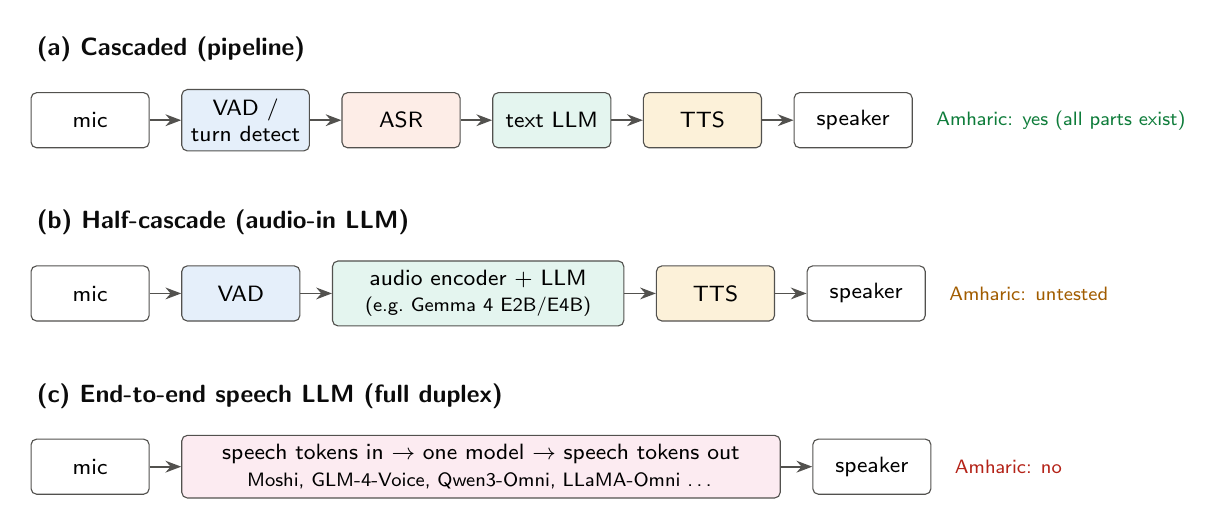
\begin{tikzpicture}[
  font=\sffamily\footnotesize, node distance=4mm,
  blk/.style={draw=ink2, rounded corners=2pt, minimum height=7mm, minimum width=15mm, align=center, fill=white},
  arr/.style={-{Stealth[length=2mm]}, ink2, semithick},
  lab/.style={font=\sffamily\small\bfseries, anchor=west, text=ink}]
% cascade
\node[lab] at (-0.2,0.9) {(a) Cascaded (pipeline)};
\node[blk] (m1) at (0.6,0) {mic};
\node[blk, right=of m1, fill=s1!12] (v1) {VAD /\\turn detect};
\node[blk, right=of v1, fill=s2!12] (a1) {ASR};
\node[blk, right=of a1, fill=s3!12] (l1) {text LLM};
\node[blk, right=of l1, fill=s4!15] (t1) {TTS};
\node[blk, right=of t1] (p1) {speaker};
\foreach \x/\y in {m1/v1,v1/a1,a1/l1,l1/t1,t1/p1} \draw[arr] (\x) -- (\y);
\node[anchor=west, text=good, font=\sffamily\scriptsize] at (p1.east) {\ \ Amharic: yes (all parts exist)};
% half cascade
\node[lab] at (-0.2,-1.3) {(b) Half-cascade (audio-in LLM)};
\node[blk] (m2) at (0.6,-2.2) {mic};
\node[blk, right=of m2, fill=s1!12] (v2) {VAD};
\node[blk, right=of v2, minimum width=37mm, fill=s3!12] (l2) {audio encoder + LLM\\{\scriptsize (e.g.\ Gemma 4 E2B/E4B)}};
\node[blk, right=of l2, fill=s4!15] (t2) {TTS};
\node[blk, right=of t2] (p2) {speaker};
\foreach \x/\y in {m2/v2,v2/l2,l2/t2,t2/p2} \draw[arr] (\x) -- (\y);
\node[anchor=west, text=warnc, font=\sffamily\scriptsize] at (p2.east) {\ \ Amharic: untested};
% end-to-end
\node[lab] at (-0.2,-3.5) {(c) End-to-end speech LLM (full duplex)};
\node[blk] (m3) at (0.6,-4.4) {mic};
\node[blk, right=of m3, minimum width=76mm, fill=s5!15] (e3) {speech tokens in $\rightarrow$ one model $\rightarrow$ speech tokens out\\{\scriptsize Moshi, GLM-4-Voice, Qwen3-Omni, LLaMA-Omni \dots}};
\node[blk, right=of e3] (p3) {speaker};
\draw[arr] (m3) -- (e3); \draw[arr] (e3) -- (p3);
\node[anchor=west, text=bad, font=\sffamily\scriptsize] at (p3.east) {\ \ Amharic: no};
\end{tikzpicture}
\caption{The three system families. Only the cascade can be built for Amharic with open weights
today. The half-cascade depends on whether an audio-input LLM understands Amharic speech, which is
still to be tested (experiment E-HC-1).}
\label{fig:families}
\end{figure}

\subsection{(a) Cascaded pipelines}
A voice-activity detector (VAD) finds speech; a turn detector decides that the user has finished;
automatic speech recognition (ASR) turns audio into text; a text LLM writes the reply; text-to-speech
(TTS) turns it back into audio. Every component can be swapped independently, and every stage can
be measured separately, which is exactly what the assignment requires. The cost is that latency
\emph{adds up}, unless the stages overlap.

\paragraph{Sequential vs.\ streaming cascades.}
The naive cascade waits for each stage to finish before starting the next. A \emph{streaming}
cascade passes partial results forward as soon as they exist:
\begin{itemize}
  \item \textbf{Streaming ASR} emits partial transcripts while the user is still talking, so at the
  endpoint only the last few hundred milliseconds of audio remain to decode. CTC encoders do this
  by processing overlapping chunks. Whisper can be forced into it with the \emph{LocalAgreement}
  policy~\cite{machacek2023}, at the cost of roughly 3\,s lag on GPU. Qwen3-ASR has a native
  2-second-chunk streaming mode~\cite{qwen3asr}.
  \item \textbf{Streaming LLM} output is standard: tokens arrive one by one. The important quantities
  are time to first token (TTFT, dominated by \emph{prefill} of the prompt) and time to the first
  \emph{speakable} chunk, meaning the first clause boundary.
  \item \textbf{Chunked or streaming TTS} synthesises the first clause while the LLM writes the next.
  Non-autoregressive models (VITS, diffusion) must wait for a whole chunk of text. Codec-LM TTS
  (e.g.\ Orpheus with SNAC) can emit audio frames incrementally.
\end{itemize}
Figure~\ref{fig:timeline} shows why this matters: in the streaming version, \ttfa\ contains only the
\emph{head} of each stage, not its full duration.

\begin{figure}[H]
\centering
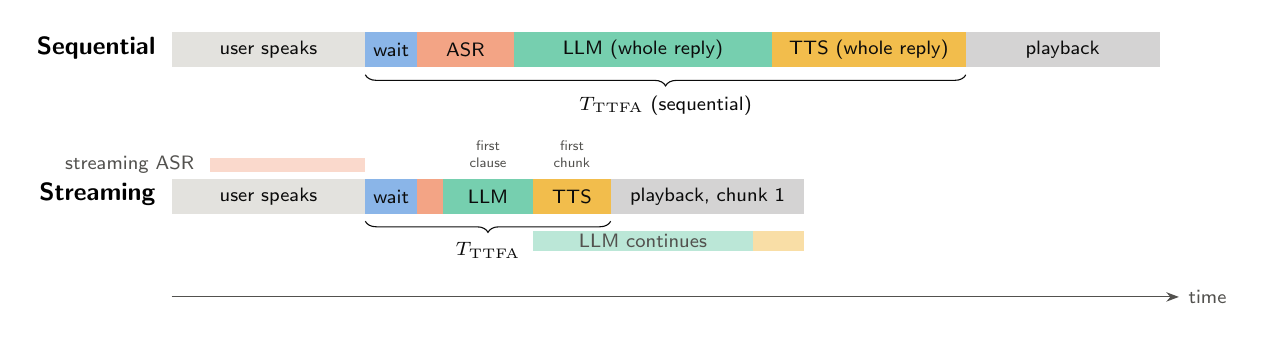
\begin{tikzpicture}[font=\sffamily\scriptsize, x=0.82cm, y=0.62cm]
\def\row#1#2#3#4#5{\fill[#4] (#1,#2) rectangle (#3,#2+0.72); \node[anchor=center, text=ink] at ({(#1+#3)/2},#2+0.36) {#5};}
% axis
\draw[ink2, -{Stealth[length=1.6mm]}] (0,-0.4) -- (15.6,-0.4) node[anchor=west] {time};
% --- sequential
\node[anchor=east, font=\sffamily\small\bfseries] at (-0.1,4.7) {Sequential};
\row{0}{4.3}{3}{rule}{user speaks}
\row{3}{4.3}{3.8}{s1!55}{wait}
\row{3.8}{4.3}{5.3}{s2!60}{ASR}
\row{5.3}{4.3}{9.3}{s3!60}{LLM (whole reply)}
\row{9.3}{4.3}{12.3}{s4!70}{TTS (whole reply)}
\row{12.3}{4.3}{15.3}{ink2!25}{playback}
\draw[decorate, decoration={brace, amplitude=4pt, mirror}, ink] (3,4.15) -- (12.3,4.15) node[midway, below=4pt] {\ttfa\ (sequential)};
% --- streaming
\node[anchor=east, font=\sffamily\small\bfseries] at (-0.1,1.7) {Streaming};
\row{0}{1.3}{3}{rule}{user speaks}
\fill[s2!25] (0.6,2.15) rectangle (3,2.45); \node[anchor=east, text=ink2] at (0.5,2.3) {streaming ASR};
\row{3}{1.3}{3.8}{s1!55}{wait}
\row{3.8}{1.3}{4.2}{s2!60}{}
\row{4.2}{1.3}{5.6}{s3!60}{LLM}
\row{5.6}{1.3}{6.8}{s4!70}{TTS}
\row{6.8}{1.3}{9.8}{ink2!25}{playback, chunk 1}
\node[anchor=south, text=ink2, font=\sffamily\tiny, align=center] at (4.9,2.05) {first\\clause};
\node[anchor=south, text=ink2, font=\sffamily\tiny, align=center] at (6.2,2.05) {first\\chunk};
\fill[s3!30] (5.6,0.55) rectangle (9.0,0.95); \node[text=ink2] at (7.3,0.75) {LLM continues};
\fill[s4!35] (9.0,0.55) rectangle (9.8,0.95);
\draw[decorate, decoration={brace, amplitude=4pt, mirror}, ink] (3,1.15) -- (6.8,1.15) node[midway, below=4pt] {\ttfa};
\end{tikzpicture}
\caption{Same components, two orchestrations (schematic, not to scale). Streaming moves ASR work
before the endpoint and overlaps LLM and TTS generation with playback. \ttfa\ then depends on the
endpoint wait, the tail of ASR, LLM time to first clause and TTS time for that clause.}
\label{fig:timeline}
\end{figure}

\subsection{(b) Half-cascades: audio-in LLMs}
Some recent LLMs accept audio directly and can answer spoken questions without a separate ASR step.
Among open models, Gemma~4 E2B/E4B include a $\sim$300M-parameter audio encoder, support ASR and
speech translation for audio up to 30\,s, and were pre-trained on 140+ languages~\cite{gemma4card}.
The model card does not say whether its audio understanding covers Amharic. If it does, the
ASR stage disappears, and so does the separate transcript decode that is very slow for Amharic
(Section~\ref{sec:m-tok}). This is a high-value, low-cost test (E-HC-1).

\subsection{(c) End-to-end speech LLMs}
Full-duplex models such as Moshi~\cite{moshi} (about 200\,ms practical latency),
LLaMA-Omni~\cite{llamaomni}, GLM-4-Voice~\cite{glm4voice} and Qwen3-Omni~\cite{qwen3omni} model
speech tokens directly and can respond while the user is still talking. They represent the lowest
latency possible in principle, but none of them produces Amharic speech. SeamlessM4T~v2 accepts
Amharic speech but outputs Amharic only as \emph{text}, not speech~\cite{seamless}. Training such a
model for Amharic is well beyond a two-week budget. \textbf{Conclusion: the realistic architecture is
a streaming cascade, possibly a half-cascade, and the work is making every head of every stage
short.}

\subsection{Turn-taking: the stage everyone underestimates}
\label{sec:how-turn}
A VAD such as Silero~\cite{silero} tells speech from silence in under a millisecond per 32\,ms
frame, but it cannot tell a \emph{thinking pause} from the \emph{end of a turn}. Pure-silence
endpointers therefore wait a fixed \emph{hangover} (often 300--800\,ms~\cite{webrtcventures2026}),
and that wait is added directly to \ttfa. There are two ways to shorten it:
\begin{itemize}
  \item \textbf{Semantic end-of-turn models}, which judge from prosody or words whether the speaker
  is done. Smart Turn v3 uses a Whisper-tiny encoder with an 8M-parameter classifier on the last 8\,s
  of audio, and covers 14 languages (not Amharic)~\cite{smartturn}. Text-based detectors run a small
  LM on the partial transcript.
  \item \textbf{Speculative response}: start ASR finalisation and LLM prefill at the \emph{first}
  short pause, and throw the work away if the user continues. This hides the endpoint wait whenever
  the guess is right.
\end{itemize}

\subsection{Where production systems spend their time}
Industry latency budgets for (English) voice agents in 2026 put turn detection at 150--400\,ms,
streaming ASR finalisation at 100--300\,ms, LLM TTFT at 250--500\,ms and TTS first audio at
100--200\,ms, for a total of about 0.6--1.2\,s~\cite{webrtcventures2026,deepgram2026}. The two
consistently largest items are \textbf{turn-taking} and \textbf{LLM time to first token}. Prompt
caching of a fixed system prompt typically removes 200--400\,ms of TTFT~\cite{webrtcventures2026}.
Section~\ref{sec:measure} tests how these proportions change for Amharic on a laptop CPU.

\section{What makes Amharic different (for latency and quality)}
\label{sec:amharic}

Most published latency engineering assumes English. Five properties of Amharic change the picture;
the first two are \emph{latency} problems, the rest are \emph{quality} problems that latency
optimisations can make worse.

\paragraph{1. The script is expensive for byte-level tokenizers.}
Amharic is written in the Ge'ez abugida (\textit{fidel}): each character is a consonant+vowel
syllable in the Unicode range U+1200–U+137F. UTF-8 stores each character in 3 bytes, and most
multilingual BPE vocabularies contain few Ethiopic merges. The result is that one Amharic word costs
several times more tokens than one English word, and \textbf{every extra token is an extra
autoregressive decoding step}, both in the LLM and in any Whisper-style ASR decoder. We measured this
directly (Section~\ref{sec:m-tok}): 12.2 tokens per word for Whisper and Llama~3.2, 6.5 for Qwen3,
3.3 for Gemma~3/4, and 1.7 for a Llama with an extended Amharic vocabulary.

\paragraph{2. Spontaneous Amharic speech is full of pauses.}
In the WAXAL test utterances we found 7.1 internal pauses per utterance, and the 90th percentile pause
was 480\,ms (Section~\ref{sec:m-endpoint}). A silence-only endpointer must therefore wait long, or it
cuts people off. The open semantic turn detector (Smart Turn~v3) was not trained on Amharic, and we
found that it does not transfer.

\paragraph{3. The script under-specifies pronunciation.}
Gemination (doubled consonants) and some vowel distinctions are not written, and several letters
are homophones in modern Amharic (\am{ሀ/ሐ/ኀ}, \am{ሰ/ሠ}, \am{አ/ዐ}, \am{ጸ/ፀ}). This means that
(i) ASR output is judged unfairly unless homophones are folded before computing WER. Gete et al.\
report that homophone normalisation substantially changes WER~\cite{whisperam}, and we fold them in
all our metrics (\code{smoke/am\_text.py}). It also means that (ii) TTS needs either a pronunciation
model or data that implicitly teaches gemination. MMS-TTS romanises input with \code{uroman} first,
which merges ejectives with plain consonants and ignores gemination~\cite{mms}.

\paragraph{4. Numbers, dates, time and calendar.}
Ethiopia uses its own calendar (currently year 2019~E.C.) and a 12-hour clock that starts at dawn
(``\am{ሶስት ሰዓት}'' is 9\,a.m.\ in international time). An assistant must say these correctly. Our
TTS test showed that MMS-TTS \emph{silently drops digits} (``15'', ``2019''): the round-trip CER of the
date sentence was 46\% (Section~\ref{sec:m-tts}). A number-to-words normaliser for Amharic is
therefore mandatory before any TTS. It is fast, so it costs no meaningful latency.

\paragraph{5. Code-switching and names.}
Urban Amharic mixes English words (``meeting'', ``Zoom'', ``email''). ASR models trained on
monolingual Amharic transcribe them in fidel or drop them, and TTS romanisers mispronounce them.
Our code-switched sentence had 62\% round-trip CER. Ethiopian personal and place names (\am{አበበ
በቀለ}, \am{ባህር ዳር}, \am{ላሊበላ}) are partly handled, at 22\% CER for the names sentence. The
evaluation set must contain all of these (Section~\ref{sec:eval}).

\begin{finding}[Consequence for design]
For Amharic, the choice of \emph{tokenizer} is a latency decision, and \emph{text normalisation} is a
quality requirement. A model that is fast in English can be several times slower in Amharic just
because of how many tokens it has to emit.
\end{finding}

\section{Candidate components (open weights, September 2026)}
\label{sec:components}

This section surveys the open, self-hostable candidates for each stage. For every candidate we
record quality evidence, the property that decides its latency, and whether it runs on the laptop
CPU or needs a free GPU. Section~\ref{sec:measure} gives the measurements.
WAXAL~\cite{waxal} (Google, CC-BY-4.0, released February 2026) is now the common Amharic
benchmark: about 190\,h of transcribed, image-prompted \emph{spontaneous} Amharic speech (566
training speakers), a 16\,h test set, and a TTS subset. Most numbers below refer to its test set.

\subsection{Speech recognition (ASR)}
The deciding latency property is the \textbf{decoder type}. \emph{Autoregressive} (AR) decoders
(Whisper, LLM-based ASR) emit one token per step, and Amharic needs many tokens per word. CTC decoders
emit all characters in one parallel pass, so their cost scales with audio length only. The second
property is whether the encoder can run \textbf{incrementally} while the user speaks.

\begin{table}[H]
\centering\footnotesize\setlength{\tabcolsep}{4pt}
\begin{tabularx}{\textwidth}{@{}L{3.5cm}rL{1.2cm}cY@{}}
\toprule
\textbf{Model} & \textbf{Params} & \textbf{Decoder} & \textbf{WAXAL WER/CER} & \textbf{Latency-relevant notes} \\
\midrule
Whisper large-v3, zero-shot & 1.55B & AR & 254 / 145\lit & Unusable without fine-tuning~\cite{waxalnet}. \\
MMS-1B, zero-shot & 1B & CTC & 101 / 85\lit & Unusable zero-shot~\cite{waxalnet}. \\
Omnilingual ASR 1B, zero-shot & 1B & CTC & 51.1 / 17.4\lit & 1{,}600+ languages; audio $\le$40\,s; GPU RTF 0.001--0.006 for CTC~\cite{omniasr,waxalnet}. \\
\midrule
\hfl{waxal-benchmarking/whisper-tiny-waxal-amh}{Whisper-tiny-WAXAL} & 39M & AR & 41.3 / 16.8\lit & Fast on CPU; fixed 30\,s encoder window. \\
\hfl{waxal-benchmarking/whisper-small-waxal-amh}{Whisper-small-WAXAL} & 244M & AR & 33.6 / 12.9\lit & Best Whisper option; 3.8\,s encoder floor on our CPU\meas. \\
\hfl{waxal-benchmarking/mms-300m-waxal-amh}{MMS-300M-WAXAL} & 300M & CTC & 37.8 / 13.2\lit & Cost $\propto$ audio length; chunked streaming possible. \\
\hfl{waxal-benchmarking/omniasr-ctc-300m-waxal-amh}{OmniASR-CTC-300M-WAXAL} & 300M & CTC & n/a & fairseq2 checkpoint; same family as Omnilingual. \\
Ethio-ASR (AfriHuBERT) & 94M & CTC & 30.95 / --\lit & Small and accurate; checkpoint availability to confirm~\cite{ethioasr}. \\
Ethio-ASR (MMS-1B) & 1B & CTC & 26.14 / --\lit & Larger multilingual variant~\cite{ethioasr}. \\
\hfl{badrex/Ethio-ASR-amharic}{Ethio-ASR-amharic} (w2v-BERT 2.0) & 600M & CTC & \textbf{22.37} / --\lit & Most accurate open Amharic ASR found; 2.4\,GB fp32; T4-friendly. \\
\hfl{b1n1yam/qwen3-asr-0.6b-amharic-mixed}{Qwen3-ASR-0.6B-Amharic} & 0.6B & AR (LLM) & 36.6 / 15.6\lit & Native 2\,s-chunk streaming and 92\,ms TTFT on GPU~\cite{qwen3asr}; the Qwen tokenizer costs 6.5 tokens/word\meas. \\
Whisper-large-v3-turbo Amharic (Bell) & 809M & AR (4 layers) & n/a & Gated. Cheap turbo decoder, but the large encoder is expensive on CPU. \\
Gemma~4 E2B/E4B audio encoder & $\sim$300M enc. & AR (LLM) & unknown & Half-cascade (Section~\ref{sec:how}); Amharic audio untested. \\
\bottomrule
\end{tabularx}
\caption{ASR candidates (model names link to Hugging Face). Most WAXAL numbers are from the WAXAL-NET
benchmark~\cite{waxalnet} or the model cards; WER normalisation differs between sources. Our own
numbers (Section~\ref{sec:m-asr}) use one normaliser for all models.}
\label{tab:asr-cands}
\end{table}

\paragraph{Runtimes for ASR.} CTranslate2 / faster-whisper (int8 on CPU, fp16 on GPU),
whisper.cpp (supports \code{--audio-ctx} to shrink the fixed 30\,s encoder window for short
utterances), ONNX Runtime and OpenVINO for wav2vec2-family CTC models (OpenVINO targets exactly this
kind of Intel CPU), sherpa-onnx for streaming CTC/transducer models with a built-in VAD, and vLLM for
Qwen3-ASR on GPU.

\subsection{Response generation (LLM)}
Two properties dominate latency: \textbf{time to first token} (prefill, which scales with prompt length and
model size and is largely removed by prompt caching) and \textbf{tokens per Amharic word} (decode
steps). A model that knows Amharic but emits 7 tokens per word is, on the same hardware, about twice as
slow per spoken word as one that emits 3.3.

\begin{table}[H]
\centering\footnotesize\setlength{\tabcolsep}{4pt}
\begin{tabularx}{\textwidth}{@{}L{3.6cm}L{1.7cm}cY@{}}
\toprule
\textbf{Model} & \textbf{Params} & \textbf{Tok/word}\meas & \textbf{Amharic evidence and latency notes} \\
\midrule
\hfl{rasyosef/Llama-3.2-1B-Amharic-Instruct}{Llama-3.2-1B-Amharic-Instruct} & 1.24B & \textbf{1.70} & Continued pre-training on Amharic plus an extended vocabulary. Fluent but often factually wrong in our test\meas. 14 tok/s decode on the laptop\meas. \\
Llama-3.2-400M / 180M-Amharic-Instruct & 0.4 / 0.18B & -- & Weaker. Candidate \emph{draft} models for speculative decoding if their vocabulary matches the 1B model. \\
\hfl{google/gemma-4-E2B-it}{Gemma~4 E2B-it} & 2.3B eff.\ (5.1B) & 3.26 & Pre-trained on 140+ languages~\cite{gemma4card}. Q4 GGUF 3.1\,GB. Ships an MTP draft head for speculative decoding. Amharic quality to be tested. \\
Gemma~4 E4B-it & 4.5B eff.\ (8B) & 3.26 & Stronger; realistic on a T4 in 4-bit. \\
Gemma~3 4B / 12B-it & 4 / 12B & 3.26 & Gemma~2 27B was the best open model on most AfroBench languages~\cite{afrobench}; 12B fits a T4 in 4-bit. \\
Qwen3 / Qwen3.5 & 0.6--4B & 6.48 / 7.08 & Good general ability, but about 2$\times$ the tokens of Gemma per Amharic word. \\
Qwen3.5-Amharic-4B-thinking (community) & 4B & 7.08 & Amharic fine-tune. ``Thinking'' must be off: hidden reasoning tokens delay the first spoken word. \\
Llama~3.2 (base) & 1--3B & 12.18 & Byte-level for Amharic; slow and weak. \\
Phi-4-mini & 3.8B & 9.14 & Not suitable. \\
\bottomrule
\end{tabularx}
\caption{LLM candidates. The tokens-per-word column is measured on 3{,}000 Amharic news sentences
(Section~\ref{sec:m-tok}).}
\label{tab:llm-cands}
\end{table}

\paragraph{Translation cascade (considered and rejected).} Translating Amharic$\rightarrow$English,
answering in English, and translating back (e.g.\ with NLLB) adds two sequence-to-sequence passes
before the first Amharic word exists. That adds about 2$\times$ the latency, and the rigid translations
hurt naturalness. We keep it only as a quality fallback, not as a latency candidate.

\paragraph{Runtimes for LLMs.} llama.cpp (GGUF; CPU and CUDA; prompt cache; speculative decoding
including Gemma~4 MTP heads; grammar-constrained output), vLLM and SGLang (GPU; prefix caching;
continuous batching for concurrency; fp16 on a T4, which has no bf16), and TensorRT-LLM.

\subsection{Speech synthesis (TTS)}
The deciding property is \textbf{time to first playable audio} for the first chunk. Non-autoregressive
models (VITS, diffusion) must synthesise a whole chunk before playing, so a \emph{short first chunk}
is the key lever. Codec-LM models (Orpheus + SNAC) can stream audio frame by frame, but they need
roughly 80+ codec tokens per second of audio, which means a GPU.

\begin{table}[H]
\centering\footnotesize\setlength{\tabcolsep}{4pt}
\begin{tabularx}{\textwidth}{@{}L{3.3cm}rL{2.8cm}Y@{}}
\toprule
\textbf{Model} & \textbf{Params} & \textbf{Architecture} & \textbf{Notes} \\
\midrule
\hfl{facebook/mms-tts-amh}{MMS-TTS-amh} & 36M & VITS (non-autoregressive) & Input romanised with \code{uroman}; CC-BY-NC-4.0 (non-commercial). RTF 0.57 on the laptop\meas. Drops digits and mispronounces English\meas. \\
\hfl{african-low-resource/omnivoice-amharic}{OmniVoice-Amharic} (Gheero-Leyu fork: \hfl{gheero-Leyu/amharic-omnivoice-tts}{link}) & 613M & Discrete diffusion (Qwen3-0.6B + HiggsAudioV2 codec) & Trained on $\sim$331\,h of Amharic; zero-shot voice cloning from 10\,s; Apache-2.0; about 3\,GB VRAM on a T4. The base OmniVoice reaches RTF 0.025 on an H100 with 32 steps, and 16 steps is faster~\cite{omnivoice}. MOS and CER are still ``TBD'' on the card. \\
\hfl{Bmancman/amharic-get-tts}{Orpheus-3B-Amharic} (+ GGUF) & 3B & LLM $\rightarrow$ SNAC codec tokens & True frame-level streaming; needs a strong GPU for real time; 6.6\,GB. \\
\hfl{AddisuSeteye/speecht5_tts_amharic}{SpeechT5-Amharic} & 144M & SpeechT5 + HiFi-GAN & Trained on ALFFA; autoregressive spectrogram decoder. \\
Piper voice trained on WAXAL-TTS & $\sim$20M & VITS (ONNX) & No Amharic voice exists yet. Piper is built for fast CPU inference, so this is a strong candidate for the CPU path (E-TTS-6). \\
\bottomrule
\end{tabularx}
\caption{TTS candidates. The Gheero-Leyu fork of OmniVoice-Amharic suggests it may already be the
organisation's preferred voice. Its speed on a T4 is the most important unknown for Week~7.}
\label{tab:tts-cands}
\end{table}

\subsection{VAD and turn detection}
\begin{itemize}
  \item \textbf{Silero VAD} (MIT; 2\,MB ONNX): 0.22\,ms per 32\,ms frame on the laptop\meas. Negligible cost.
  \item \textbf{TEN VAD}: a newer low-latency VAD that claims faster speech-to-silence transitions; worth a direct comparison.
  \item \textbf{Smart Turn v3.2} (BSD-2; 8M params; Whisper-tiny encoder): audio-only semantic end-of-turn
  for 14 languages. 120\,ms per call on our CPU\meas; \textbf{does not work on Amharic}\meas\ (Section~\ref{sec:m-endpoint}).
  Its training code is open, so an Amharic fine-tune on WAXAL is feasible (E-EP-3).
  \item \textbf{Text-based end-of-utterance models}: a small LM scores whether the partial transcript
  is a complete sentence. They need an Amharic model, which could be the 180M Amharic Llama.
\end{itemize}

\subsection{Orchestration and transport}
\textbf{Pipecat} (Python; frame-based pipelines; built-in interruption handling, Smart Turn and Silero
integration) and \textbf{LiveKit Agents} (WebRTC) are the open frameworks used in production voice
agents. A plain \code{asyncio} WebSocket server with 20\,ms 16\,kHz PCM frames is simpler and makes
every millisecond visible. For a single-machine demo, in-process queues avoid all network cost. Our
recommendation is to build the measurement harness on plain asyncio, and to adopt Pipecat only if its
interruption handling saves real work.

\section{Compute available for free}
\label{sec:compute}

The hardware decides which models are candidates at all, so it is treated as a design variable, not a
given. Free-tier limits change often; the numbers below were collected in September 2026 from
provider pages and 2026 guides~\cite{kagglegpu,colabfaq,lightningfree} and must be re-checked on
sign-up.

\begin{table}[H]
\centering\small
\begin{tabularx}{\textwidth}{@{}L{2.7cm}L{3.4cm}L{3.3cm}Y@{}}
\toprule
\textbf{Option} & \textbf{Hardware} & \textbf{Limits} & \textbf{Best use in this project} \\
\midrule
Laptop (ours) & i5-6300U, 2C/4T, AVX2 (no AVX-512 / VNNI), 15\,GB RAM, $\sim$2–5\,GB free disk & None; always available & The ``edge'' configuration. Every measurement in Section~\ref{sec:measure}. Final demo client (microphone and loudspeaker). \\
Kaggle Notebooks & 2$\times$T4 (16\,GB each) or 1$\times$P100 & $\sim$30 GPU-h/week; sessions capped (9–12\,h); internet after phone verification & Main GPU benchmark machine: the same notebook reruns every experiment on the same hardware. \\
Google Colab (free) & T4 16\,GB (when available) & Dynamic quota; idle timeout; $\le$12\,h sessions & Second GPU, OmniVoice demo notebook, quick checks. \\
Lightning AI Studio (free tier) & T4/L4 via monthly credits; 1 persistent CPU studio & Monthly credit allowance (sources report 22–80 GPU-h/month) & Persistent environment. Exposing a port for a live demo is simpler than on Kaggle or Colab. \\
Hugging Face Spaces & CPU basic (free); ZeroGPU needs PRO to host & Cold starts; queueing & Public demo of the CPU pipeline only. \\
Oracle Cloud Always Free & 4 Arm Ampere OCPU, 24\,GB RAM & Always on & Optional always-on CPU server (llama.cpp performs well on Arm NEON). \\
AWS SageMaker Studio Lab & – & Reported closed to new users in July 2026 & Not relied on. \\
\bottomrule
\end{tabularx}
\caption{Free compute options. A T4 (Turing, 65 TFLOPS fp16, 320\,GB/s, no bf16) is the realistic
GPU target: all fp16/int8 paths must work without bf16.}
\label{tab:compute}
\end{table}

\paragraph{The network is part of \ttfa.} If the models run in a notebook in a US data centre and the
microphone is in Addis Ababa, every turn pays at least one round trip for the user's audio and one
for the response audio, plus any tunnel overhead (cloudflared, ngrok). This must be measured
(experiment E-SYS-4). The design rule is to \textbf{co-locate all models on one machine} and to stream
audio \emph{while the user speaks}, so that uploading the user's audio overlaps with speaking and
only the response direction costs latency.

\paragraph{Two target configurations.} We therefore optimise two configurations and report both:
\begin{enumerate}
  \item \textbf{CPU-only (edge)}: the laptop, no network. This is the hardest case and the most honest one,
  and everything in Section~\ref{sec:measure} was measured here.
  \item \textbf{Single T4 (server)}: all models on one Kaggle or Colab T4, with the laptop as a thin
  audio client. This is the configuration most likely to reach the ``Good'' tier.
\end{enumerate}

\section{Measurements on the laptop CPU}
\label{sec:measure}

\subsection{Setup}
\begin{itemize}
  \item \textbf{Hardware:} Intel Core i5-6300U (Skylake, 2 cores / 4 threads, 2.4\,GHz, AVX2, no AVX-512/VNNI), 16\,GB RAM, no GPU.
  \item \textbf{Software:} Python 3.12, PyTorch 2.13 (CPU), transformers 5.15, CTranslate2 4.8.2 (faster-whisper 1.2.1),
  ONNX Runtime 1.30, llama.cpp build b11179, uroman 1.3.1, jiwer 4.0.
  \item \textbf{ASR dev data:} 30 utterances from the WAXAL Amharic test split, spread across the split
  with at most 2 per speaker (19 speakers, both genders, 519\,s, median 16.9\,s).
  \item \textbf{End-to-end turns:} 5 Amharic questions (Appendix~\ref{app:turns}), synthesised with MMS-TTS
  and padded with 0.3\,s of leading and 1.5\,s of trailing silence (2.9--4.4\,s of speech).
  \item \textbf{Normalisation:} all WER/CER numbers use \code{am\_text.normalize} (NFC, punctuation removed,
  homophone rows folded).
\end{itemize}

\subsection{Tokenizer cost of Amharic}
\label{sec:m-tok}
We encoded 3{,}000 random sentences from the Week-4 Amharic news corpus (14.3 words per sentence on
average) and the 30 WAXAL transcripts with each candidate's tokenizer.

\begin{figure}[H]
\centering
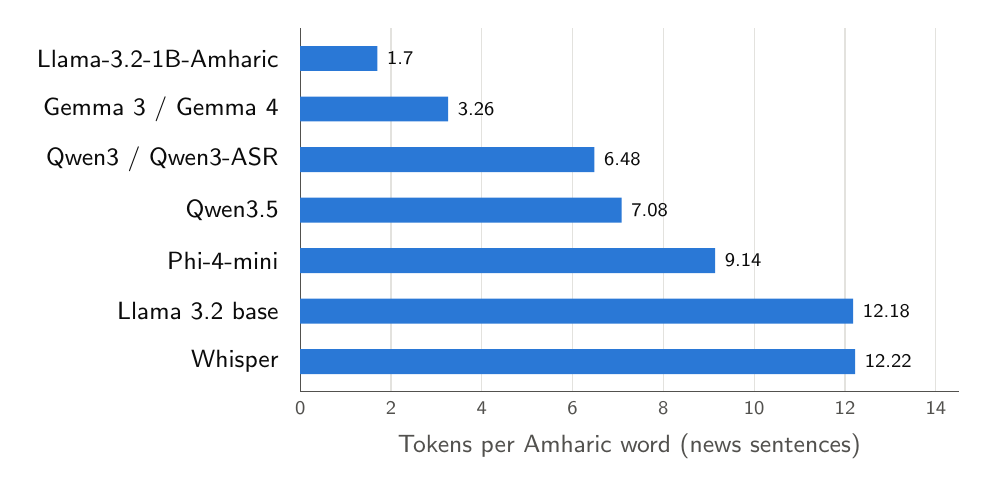
\begin{tikzpicture}
\begin{axis}[
  xbar, width=0.82\textwidth, height=6.2cm, bar width=9pt,
  xmin=0, xmax=14.5, xlabel={Tokens per Amharic word (news sentences)},
  symbolic y coords={Llama-3.2-1B-Amharic,Gemma 3 / Gemma 4,Qwen3 / Qwen3-ASR,Qwen3.5,Phi-4-mini,Llama 3.2 base,Whisper},
  ytick=data, y dir=reverse, enlarge y limits=0.1,
  axis line style={draw=ink2}, tick style={draw=none}, yticklabel style={font=\sffamily\small, text=ink},
  xticklabel style={font=\sffamily\scriptsize, text=ink2}, xlabel style={font=\sffamily\small, text=ink2},
  xmajorgrids, grid style={draw=rule}, axis x line*=bottom, axis y line*=left,
  nodes near coords, nodes near coords style={font=\sffamily\scriptsize, text=ink, anchor=west},
  every node near coord/.append style={/pgf/number format/fixed, /pgf/number format/precision=2},
]
\addplot[fill=s1, draw=none, rounded corners=0pt] coordinates {
  (1.70,Llama-3.2-1B-Amharic) (3.26,Gemma 3 / Gemma 4) (6.48,Qwen3 / Qwen3-ASR) (7.08,Qwen3.5)
  (9.14,Phi-4-mini) (12.18,Llama 3.2 base) (12.22,Whisper)};
\end{axis}
\end{tikzpicture}
\caption{Tokens per Amharic word\meas. English costs 1.1--1.2 tokens per word with all of these
tokenizers, so Amharic is 1.4$\times$ (extended-vocabulary Llama) to 10.3$\times$ (Whisper, Llama base)
more expensive. On the WAXAL speech transcripts the numbers are 3--12\% lower but in the same order.}
\label{fig:fertility}
\end{figure}

\begin{finding}[Finding 1 — the tokenizer is a latency decision]
A 30-word Amharic answer costs 51 decode steps with the Amharic Llama, 98 with Gemma, 194 with Qwen3
and 365 with base Llama. The same holds for ASR: the WAXAL Whisper models emit 18.6 tokens per second of
audio (Table~\ref{tab:asr-meas}), so a 5\,s question needs about 45 sequential decoder steps. This
explains why every Whisper variant is slow here, and why CTC is attractive.
\end{finding}

\subsection{Speech recognition}
\label{sec:m-asr}
\begin{table}[H]
\centering\footnotesize\setlength{\tabcolsep}{4pt}
\begin{tabular}{@{}lllrrrrr@{}}
\toprule
\textbf{Model} & \textbf{Runtime} & \textbf{Dec.} & \textbf{WER} & \textbf{CER} & \textbf{Latency med/p90 (s)} & \textbf{RTF} & \textbf{Turn (s)} \\
\midrule
Whisper-tiny-WAXAL & HF fp32 & AR & 38.7 & 18.3 & 7.82 / 8.99 & 0.45 & -- \\
Whisper-tiny-WAXAL & CT2 int8 & AR & 38.9 & 19.0 & \textbf{3.03} / 3.59 & \textbf{0.18} & \textbf{1.0} \\
Whisper-small-WAXAL & HF fp32$^\dagger$ & AR & 27.6 & 11.6 & 37.9 / 40.9 & 2.17 & -- \\
Whisper-small-WAXAL & CT2 int8 & AR & \textbf{29.4} & 13.0 & 14.57 / 16.58 & 0.84 & 5.6 \\
MMS-300M-WAXAL & HF fp32 & CTC & 31.4 & \textbf{12.7} & 10.79 / 20.43 & 0.63 & 2.4 \\
MMS-300M-WAXAL & + dynamic int8 & CTC & 33.7 & 13.4 & 15.56 / 19.88 & 0.91 & -- \\
\bottomrule
\end{tabular}
\caption{ASR on 30 WAXAL test utterances (median 16.9\,s) on the laptop, 4 threads, greedy decoding\meas.
HF = Hugging Face transformers. ``Turn'' is the median ASR time inside the end-to-end runs (2.9--4.4\,s questions).
$^\dagger$Only 8 utterances (too slow for the full set).}
\label{tab:asr-meas}
\end{table}

\begin{finding}[Finding 2 — what the ASR numbers say]
\textbf{(a)} CTranslate2 int8 is 2.6$\times$ faster than HF fp32 for Whisper, with no accuracy loss.
\textbf{(b)} Whisper-small and MMS-300M-CTC are equally accurate (CER 13.0 vs 12.7), but on short turns
CTC is 2.3$\times$ faster (2.4\,s vs 5.6\,s). The reason is that Whisper always encodes a padded 30\,s
window: for a 5\,s question the encoder alone takes 3.8\,s (small) or 0.55\,s (tiny), and the decoder adds
1.9\,s (38\,ms per token $\times$ 45 tokens)\meas. \textbf{(c)} PyTorch dynamic int8 \emph{slows} the CTC
model down on this CPU (RTF 0.63 $\rightarrow$ 0.91) and costs 2.3 WER points: without VNNI, int8
matrix multiplies do not pay off. Try ONNX Runtime / OpenVINO instead (E-ASR-6).
\end{finding}

\begin{caveat}[Pitfall found: faster-whisper truncates Amharic]
faster-whisper caps generation at 448 positions, and CTranslate2's Whisper \code{generate()} returned
only \code{max\_length}/2 tokens. As a result, \emph{every} transcript stopped at 224 tokens
($\approx$18 Amharic words), and WER looked like 57\% instead of 39\%. We bypass it by calling
\code{generate(max\_length=880)} directly (\code{smoke/asr\_bench.py}). Any team using faster-whisper
for Amharic should check for this.
\end{caveat}

\subsection{Endpointing}
\label{sec:m-endpoint}
Silero VAD (ONNX, 1 thread) costs \textbf{0.22\,ms per 32\,ms frame}\meas: 0.8\% of real time, which is
negligible. The problem is deciding \emph{when} the user is done. Inside the 30 WAXAL utterances we found
7.1 internal pauses per utterance, with pause lengths p50 = 160\,ms, p90 = 480\,ms and p99 = 892\,ms\meas.

\begin{figure}[H]
\centering
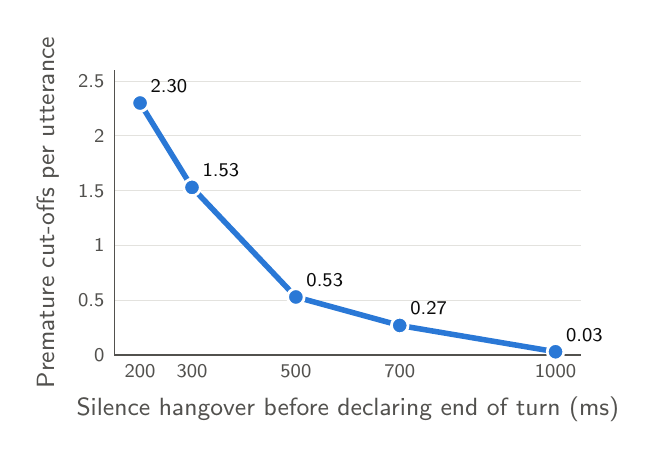
\begin{tikzpicture}
\begin{axis}[
  width=0.62\textwidth, height=5.2cm, xmin=150, xmax=1050, ymin=0, ymax=2.6,
  xlabel={Silence hangover before declaring end of turn (ms)}, ylabel={Premature cut-offs per utterance},
  xtick={200,300,500,700,1000}, ytick={0,0.5,1,1.5,2,2.5},
  axis line style={draw=ink2}, tick style={draw=none}, ymajorgrids, grid style={draw=rule},
  xticklabel style={font=\sffamily\scriptsize, text=ink2}, yticklabel style={font=\sffamily\scriptsize, text=ink2},
  xlabel style={font=\sffamily\small, text=ink2}, ylabel style={font=\sffamily\small, text=ink2},
  axis x line*=bottom, axis y line*=left,
  nodes near coords, point meta=explicit symbolic, nodes near coords style={font=\sffamily\scriptsize, text=ink, anchor=south west},
]
\addplot[s1, line width=2pt, mark=*, mark size=3pt, mark options={fill=s1, draw=white, line width=1pt}]
  coordinates {(200,2.30)[2.30] (300,1.53)[1.53] (500,0.53)[0.53] (700,0.27)[0.27] (1000,0.03)[0.03]};
\end{axis}
\end{tikzpicture}
\caption{How often a pure-silence endpointer would cut a speaker off mid-utterance, as a function of
the hangover\meas. Data: 30 spontaneous WAXAL utterances, averaging 17\,s. Shorter conversational
questions will have fewer pauses (E-EP-1).}
\label{fig:hangover}
\end{figure}

We then tested \textbf{Smart Turn v3.2} (CPU ONNX) at the true end of each utterance and at each of
69 internal pauses of at least 200\,ms. It returned P(complete) with a median of 0.94 at true ends,
\emph{but 0.95 at mid-utterance pauses}: 84\% of internal pauses were classified as ``turn complete''\meas.
Each call took 120\,ms on this CPU (the authors report 12\,ms on modern CPUs~\cite{smartturn}).

\begin{finding}[Finding 3 — endpointing is a first-class bottleneck]
With silence only, a safe hangover for spontaneous Amharic is 700--1000\,ms of pure waiting. That is
already more than an entire English voice agent's LLM budget. The off-the-shelf semantic detector does
not understand Amharic. An Amharic end-of-turn model (E-EP-3, E-EP-4) and speculative turn-ending
(E-EP-5) are therefore among the highest-value experiments, and they help equally on CPU and GPU.
\end{finding}

\subsection{Response generation}
\label{sec:m-llm}
Model: \hf{rasyosef/Llama-3.2-1B-Amharic-Instruct}, GGUF Q4\_K\_M (825\,MB), llama.cpp server,
context 2{,}048, temperature 0.3.

\begin{table}[H]
\centering\small
\begin{tabular}{@{}lrr@{}}
\toprule
\textbf{llama-bench} & \textbf{2 threads} & \textbf{4 threads} \\
\midrule
Prompt processing, 128 / 512 tokens (tok/s) & 46.0 / 45.3 & 45.2 / 45.5 \\
Generation, 64 tokens (tok/s) & \textbf{14.2} & 12.8 \\
\bottomrule
\end{tabular}

\vspace{6pt}
\begin{tabular}{@{}lrr@{}}
\toprule
\textbf{Streaming, 5 questions (median)} & \textbf{cold} & \textbf{warm} \\
\midrule
Prompt tokens / prefill (ms) & 61 / 1{,}490 & 11 / 396 \\
Time to first token (ms) & 1{,}504 & \textbf{416} \\
Time to first clause (ms) & 2{,}584 & \textbf{1{,}378} \\
Tokens per word of replies & \multicolumn{2}{c}{1.6} \\
\bottomrule
\end{tabular}
\caption{LLM on the laptop CPU\meas. ``Warm'' = system prompt cached in the KV cache, question not
cached. Hyper-threading hurts decoding (2 threads beat 4).}
\label{tab:llm-meas}
\end{table}

\begin{finding}[Finding 4 — the LLM is fast enough on CPU, but not good enough]
At 14 tokens/s and 1.6 tokens per word, the 1B Amharic model generates about 8 words/s, faster than
speech, and prompt caching cuts TTFT from 1.5\,s to 0.42\,s. \textbf{Quality is the limit}: replies are
fluent Amharic but often wrong or off-topic. Examples: it claimed coffee is ``4--5\% salt'', put
``pizza'' in a coffee answer, and after an ASR error answered that Ethiopia's capital is ``Manhattan''.
It also ignores the ``one or two sentences'' instruction (up to 82 words). Relevance, not speed,
decides the LLM (E-LLM-2).
\end{finding}

\subsection{Speech synthesis}
\label{sec:m-tts}
\begin{table}[H]
\centering\small
\begin{tabular}{@{}lrrrrr@{}}
\toprule
\textbf{Sentence} & \textbf{Words} & \textbf{Audio (s)} & \textbf{Synthesis (ms)} & \textbf{RTF} & \textbf{Round-trip CER} \\
\midrule
greeting & 4 & 2.94 & 1{,}536 & 0.52 & 5.0\% \\
capital & 6 & 4.13 & 2{,}246 & 0.54 & 4.2\% \\
weather & 12 & 6.91 & 3{,}920 & 0.57 & 12.8\% \\
museum hours (Ethiopian time) & 12 & 5.76 & 3{,}380 & 0.59 & 16.7\% \\
names and places & 18 & 10.75 & 6{,}195 & 0.58 & 22.0\% \\
digits and date & 9 & 3.81 & 2{,}121 & 0.56 & \textcolor{bad}{\textbf{46.2\%}} \\
code-switching & 12 & 5.42 & 3{,}094 & 0.57 & \textcolor{bad}{\textbf{62.5\%}} \\
\bottomrule
\end{tabular}
\caption{MMS-TTS (VITS, 36M parameters, 16\,kHz) on the laptop, 2 threads, median of 3 runs\meas. Round-trip
CER = CER of Whisper-small-WAXAL transcribing the synthesised audio (lower is more intelligible). 4 threads
gave no gain (RTF 0.59). Loading takes 9.8\,s, and the first call is slower (lazy initialisation).}
\label{tab:tts-meas}
\end{table}

\begin{finding}[Finding 5 — TTS: short first chunks and text normalisation]
VITS cost is linear in output length (RTF $\approx$ 0.57), so the first audio of a 4-word chunk takes
about 1.5\,s and a whole 40-word reply about 14\,s. Chunking is therefore mandatory on CPU. The digits
``15'' and ``2019'' are silently dropped (the romanised vocabulary has no digits), and English words
come out unintelligible (``Zoom'' $\rightarrow$ \am{በጾም}). A normaliser is required (E-TTS-3).
\end{finding}

\subsection{End-to-end baseline}
\label{sec:m-e2e}
The harness (\code{smoke/e2e\_baseline.py}) streams each user turn through Silero VAD with a 700\,ms
hangover, transcribes up to the endpoint, streams the LLM, and synthesises in one of three modes:
\textbf{A} sequential (whole reply), \textbf{B} first clause (first clause mark after $\geq$2 words),
\textbf{C} first clause \emph{or} 5 words, whichever comes first. In B and C the LLM keeps generating in
parallel while the first chunk is synthesised, so the two compete for the same 2 cores, as they would in
a real system. LLM: 2 threads; TTS: 2 threads.

\begin{figure}[H]
\centering
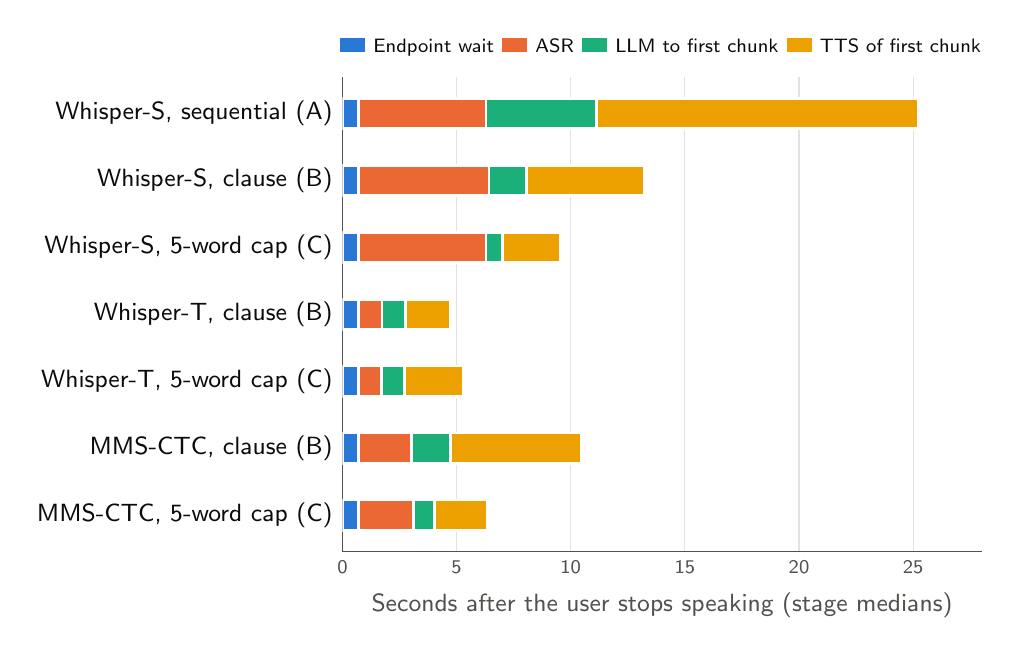
\begin{tikzpicture}
\begin{axis}[
  xbar stacked, width=0.80\textwidth, height=7.6cm, bar width=11pt,
  xmin=0, xmax=28, xlabel={Seconds after the user stops speaking (stage medians)},
  symbolic y coords={A,B,C,D,E,F,G}, ytick=data, y dir=reverse, enlarge y limits=0.09,
  yticklabels={{Whisper-S, sequential (A)}, {Whisper-S, clause (B)}, {Whisper-S, 5-word cap (C)},
               {Whisper-T, clause (B)}, {Whisper-T, 5-word cap (C)}, {MMS-CTC, clause (B)}, {MMS-CTC, 5-word cap (C)}},
  yticklabel style={font=\sffamily\small, text=ink}, xticklabel style={font=\sffamily\scriptsize, text=ink2},
  xlabel style={font=\sffamily\small, text=ink2}, axis line style={draw=ink2}, tick style={draw=none},
  xmajorgrids, grid style={draw=rule}, axis x line*=bottom, axis y line*=left,
  legend style={font=\sffamily\scriptsize, draw=none, fill=none, at={(0.5,1.02)}, anchor=south, legend columns=4, text=ink},
  legend image code/.code={\fill[#1] (0cm,-0.08cm) rectangle (0.35cm,0.14cm);},
]
\addplot[fill=s1, draw=white, line width=1pt] coordinates {(0.70,A) (0.70,B) (0.70,C) (0.70,D) (0.70,E) (0.70,F) (0.70,G)};
\addplot[fill=s2, draw=white, line width=1pt] coordinates {(5.59,A) (5.72,B) (5.59,C) (1.03,D) (1.02,E) (2.34,F) (2.41,G)};
\addplot[fill=s3, draw=white, line width=1pt] coordinates {(4.83,A) (1.64,B) (0.72,C) (1.02,D) (0.99,E) (1.69,F) (0.91,G)};
\addplot[fill=s4, draw=white, line width=1pt] coordinates {(14.11,A) (5.17,B) (2.52,C) (1.96,D) (2.58,E) (5.72,F) (2.33,G)};
\legend{Endpoint wait, ASR, LLM to first chunk, TTS of first chunk}
\end{axis}
\end{tikzpicture}
\caption{Where the time goes, per configuration (medians of each stage over 5 turns)\meas. Whisper-S /
Whisper-T = Whisper small / tiny WAXAL (CT2 int8); MMS-CTC = MMS-300M-WAXAL (fp32); LLM = Amharic Llama 1B
Q4\_K\_M; TTS = MMS-TTS. Median \ttfa\ per row is given in Table~\ref{tab:e2e}.}
\label{fig:e2e}
\end{figure}

\begin{table}[H]
\centering\footnotesize\setlength{\tabcolsep}{4pt}
\begin{tabularx}{\textwidth}{@{}llrrrY@{}}
\toprule
\textbf{ASR} & \textbf{Mode} & \textbf{\ttfa\ median (s)} & \textbf{p90 (s)} & \textbf{min--max (s)} & \textbf{Largest stage} \\
\midrule
Whisper-small & A sequential & 25.2 & 46.3 & 7.2--50.6 & TTS of whole reply (14.1\,s) \\
Whisper-small & B clause & 13.0 & 17.5 & 9.4--18.7 & ASR (5.7\,s), TTS (5.2\,s) \\
Whisper-small & C 5-word cap & 9.2 & 10.6 & 8.7--10.8 & ASR (5.6\,s) \\
Whisper-tiny & B clause & \textbf{4.4} & 9.2 & 4.2--11.7 & TTS (2.0\,s) \\
Whisper-tiny & C 5-word cap & 5.4 & 6.4 & 4.0--6.4 & TTS (2.6\,s) \\
MMS-300M CTC & B clause & 10.8 & 15.2 & 4.5--16.4 & TTS (5.7\,s) \\
MMS-300M CTC & C 5-word cap & \textbf{5.9} & \textbf{6.8} & 4.4--6.8 & ASR (2.4\,s), TTS (2.3\,s) \\
\bottomrule
\end{tabularx}
\caption{End-to-end \ttfa\ on the laptop CPU, 5 turns per row\meas. Whisper-tiny is the fastest, but on
these turns its CER is 22.0\%, against 15.6\% for MMS-300M-CTC and 14.7\% for Whisper-small
(Appendix~\ref{app:turns}). That matches the WAXAL ranking, so MMS-300M-CTC with the 5-word cap is the
best \emph{usable} CPU configuration so far.}
\label{tab:e2e}
\end{table}

\begin{finding}[Finding 6 — streaming gives 2.7$\times$, the CTC swap another 1.6$\times$]
With the \emph{same three models} on the \emph{same laptop}, sequential processing takes 25.2\,s median
and streaming with a capped first chunk takes 9.2\,s. Swapping Whisper-small for a CTC model of equal
accuracy brings it to 5.9\,s (4.3$\times$ better than the sequential baseline). Clause-only chunking (B)
has a long tail: when the model's first sentence is long, synthesising it while the LLM is still decoding
takes 5--11\,s. The cap (C) removes that tail (p90 15.2 $\rightarrow$ 6.8\,s).
\end{finding}

\subsection{Resources}
\begin{center}\small
\begin{tabular}{@{}lrl@{}}
\toprule
\textbf{Component (loaded, after one inference)} & \textbf{RSS} & \textbf{Load time} \\
\midrule
Whisper-tiny-WAXAL, CT2 int8 & 129\,MB & $<$1\,s \\
Whisper-small-WAXAL, CT2 int8 & 551\,MB & $<$1\,s \\
MMS-300M-WAXAL CTC, fp32 & 1{,}602\,MB & 6.7\,s \\
MMS-TTS (VITS) & 167\,MB & 9.8\,s (incl.\ uroman) \\
llama.cpp server, 1B Q4\_K\_M, 2k context & 1{,}457\,MB & 2.9\,s \\
\midrule
Full CPU pipeline (CTC + LLM + TTS) & $\approx$3.2\,GB & 13\,s \\
\bottomrule
\end{tabular}
\end{center}
The whole pipeline fits comfortably in 16\,GB of RAM; memory is not a constraint on the CPU path.
Compute (2 physical cores shared by three models) is the constraint.

\section{Bottleneck analysis}
\label{sec:bottlenecks}

\subsection{Ranking on the laptop (best usable configuration)}
For the MMS-300M-CTC, 5-word-cap configuration (median \ttfa\ 5.9\,s), the stage medians are:

\begin{center}\small
\begin{tabularx}{\textwidth}{@{}L{6.2cm}rrY@{}}
\toprule
\textbf{Stage} & \textbf{Median (s)} & \textbf{Share} & \textbf{Nature of the cost} \\
\midrule
ASR after endpoint (offline CTC over the whole turn) & 2.41 & 38\% & compute; avoidable by streaming \\
TTS of the first chunk (under LLM contention) & 2.33 & 37\% & compute + contention \\
LLM to first 5 words (warm cache) & 0.91 & 14\% & compute (prefill + $\sim$8 tokens) \\
Endpoint wait (700\,ms hangover) & 0.70 & 11\% & \emph{pure waiting} \\
\bottomrule
\end{tabularx}
\end{center}
(The shares are of the sum of stage medians, 6.35\,s, which differs slightly from the median \ttfa.)

\textbf{Interpretation.}
\begin{enumerate}
  \item \textbf{ASR finalisation} is the largest term, and almost all of it is avoidable: the audio was
  available while the user spoke. Streaming CTC (E-ASR-4) should reduce it to roughly one chunk
  (0.2--0.4\,s on this CPU\proj).
  \item \textbf{First-chunk TTS} costs 2.3\,s, of which about 0.9\,s is contention. The first chunks are
  about 2.5\,s of audio, which would take about 1.4\,s on an idle CPU (RTF 0.57). While the LLM keeps
  decoding in parallel, the effective RTF rises to 0.8--1.2\meas. Contention control (E-SYS-2) and a
  faster runtime or voice (E-TTS-5/6) attack it.
  \item \textbf{The LLM} is not the latency problem on this hardware once the prompt is cached; it is the
  \emph{quality} problem.
  \item \textbf{The endpoint wait} is small in this configuration only because the other terms are large. On a
  GPU it becomes the dominant term.
\end{enumerate}

\subsection{Projected budgets after optimisation}
The table below is a \emph{projection}\proj\ built from our CPU measurements, the literature numbers in
Section~\ref{sec:components}, and the expected effect of the experiments. It is the hypothesis Week~7
has to confirm or reject, not a result.

\begin{center}\small
\begin{tabularx}{\textwidth}{@{}L{3.2cm}rrY@{}}
\toprule
\textbf{Stage} & \textbf{CPU now}\meas & \textbf{CPU target}\proj & \textbf{How} \\
\midrule
Endpoint wait & 0.70 & 0.30--0.45 & Amharic end-of-turn model + speculative start (E-EP-3/4/5) \\
ASR after endpoint & 2.41 & 0.25--0.40 & Streaming CTC during speech; ONNX/OpenVINO (E-ASR-4/6) \\
LLM to first chunk & 0.91 & 0.6--0.8 & Caching (done), spoken prompt, pinned cores (E-LLM-4/7) \\
TTS first chunk & 2.33 & 0.5--1.0 & Contention control, ONNX VITS or Piper voice (E-SYS-2, E-TTS-5/6) \\
\midrule
\textbf{\ttfa} & \textbf{5.9} & \textbf{1.7--2.7} & ``Acceptable'' tier on a 2016 laptop \\
\bottomrule
\end{tabularx}
\end{center}

\begin{center}\small
\begin{tabularx}{\textwidth}{@{}L{3.2cm}rY@{}}
\toprule
\textbf{Stage} & \textbf{T4 target}\proj & \textbf{Basis} \\
\midrule
Endpoint wait & 0.30--0.45 & Same as CPU (waiting does not get faster on a GPU) \\
ASR after endpoint & 0.05--0.15 & CTC encoders run at RTF $\sim$0.001--0.006 on GPU~\cite{omniasr}; the last streaming chunk only \\
LLM to first chunk & 0.3--0.5 & Gemma~4 E2B/E4B in 4-bit, cached prompt, $\sim$16 tokens for the first 5 words \\
TTS first chunk & 0.2--0.5 & MMS-TTS on GPU, or OmniVoice with 8--16 steps on a short chunk~\cite{omnivoice} \\
Network (laptop $\leftrightarrow$ notebook) & 0.2--0.4 & One response-direction trip plus the tunnel; to be measured (E-SYS-4) \\
\midrule
\textbf{\ttfa} & \textbf{1.1--2.0} & ``Good'' tier, with the endpoint wait and the network now dominant \\
\bottomrule
\end{tabularx}
\end{center}

\begin{finding}[Where Week 7 should spend its time]
On the CPU: ASR streaming and TTS contention first (together $\approx$75\% of \ttfa). On the GPU: the
endpoint wait and the network, because compute stops being the bottleneck. Both paths share the
Amharic end-of-turn work. That is why E-EP-3/5 are P0 even though they save less on the CPU today.
\end{finding}

\section{Baseline definition and recommended architecture}
\label{sec:baseline}

\subsection{The official baseline}
The assignment asks for improvement measured against a baseline, so the baseline must be fixed now and
never edited later.
\begin{keybox}
\textbf{Baseline B0 (frozen 25 Sep 2026).} A straightforward, non-streaming cascade using the most
accurate components that run on the laptop: Silero VAD with a 700\,ms hangover $\rightarrow$
Whisper-small-WAXAL (CT2 int8) $\rightarrow$ Llama-3.2-1B-Amharic-Instruct Q4\_K\_M (llama.cpp, 2
threads, cached system prompt) $\rightarrow$ MMS-TTS of the whole reply.
\textbf{Measured \ttfa: 25.2\,s median, 46.3\,s p90} (5 synthetic turns; to be re-measured on the recorded
conversational set, E-INF-2). The same configuration on a Kaggle T4 is baseline B0-GPU (E-INF-3).
\end{keybox}

Already measured improvements over B0 (same laptop):
\begin{center}\small
\begin{tabularx}{\textwidth}{@{}L{5.6cm}rrY@{}}
\toprule
\textbf{Change (cumulative)} & \textbf{\ttfa\ median} & \textbf{vs B0} & \textbf{Keep?} \\
\midrule
B0: sequential & 25.2\,s & -- & reference \\
+ LLM streaming, TTS of the first clause (mode B) & 13.0\,s & $-48\%$ & keep streaming; first-chunk rule changed below \\
+ first chunk capped at 5 words (mode C) & 9.2\,s & $-64\%$ & keep \\
+ ASR: Whisper-small $\rightarrow$ MMS-300M CTC (equal CER) & \textbf{5.9\,s} & $\mathbf{-77\%}$ & keep (current best) \\
\textit{Alternative:} ASR $\rightarrow$ Whisper-tiny & 5.4\,s & $-79\%$ & reject: CER 19 vs 13 (WAXAL), 22 vs 16 (turns) \\
\textit{Tried:} dynamic int8 on the CTC model & slower & -- & reject: RTF 0.63 $\rightarrow$ 0.91 \\
\bottomrule
\end{tabularx}
\end{center}

\subsection{Recommended target architecture}
\begin{figure}[H]
\centering
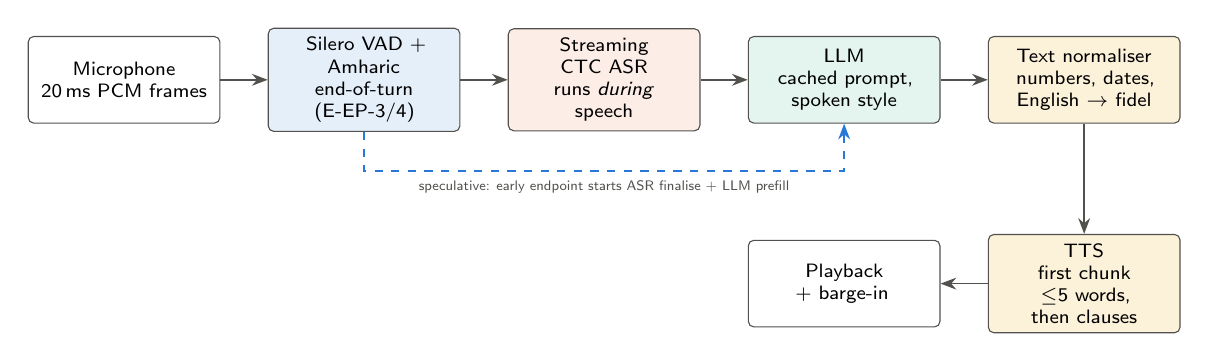
\begin{tikzpicture}[font=\sffamily\scriptsize, node distance=14mm and 6mm,
  blk/.style={draw=ink2, rounded corners=2pt, minimum height=11mm, text width=22mm, align=center, fill=white},
  arr/.style={-{Stealth[length=2mm]}, ink2, semithick}, note/.style={text=ink2, font=\sffamily\tiny}]
\node[blk] (mic) {Microphone\\20\,ms PCM frames};
\node[blk, right=of mic, fill=s1!12] (vad) {Silero VAD +\\Amharic end-of-turn\\(E-EP-3/4)};
\node[blk, right=of vad, fill=s2!12] (asr) {Streaming CTC ASR\\runs \emph{during}\\speech};
\node[blk, right=of asr, fill=s3!12] (llm) {LLM\\cached prompt,\\spoken style};
\node[blk, right=of llm, fill=s4!15] (norm) {Text normaliser\\numbers, dates,\\English $\rightarrow$ fidel};
\node[blk, below=of norm, fill=s4!15] (tts) {TTS\\first chunk $\leq$5 words,\\then clauses};
\node[blk, left=of tts] (play) {Playback\\+ barge-in};
\draw[arr] (mic) -- (vad); \draw[arr] (vad) -- (asr); \draw[arr] (asr) -- (llm);
\draw[arr] (llm) -- (norm); \draw[arr] (norm) -- (tts); \draw[arr] (tts) -- (play);
\draw[arr, dashed, s1] (vad.south) -- ++(0,-5mm) -| (llm.south);
\node[note, anchor=north] at ($(vad.south)!0.5!(llm.south) + (0,-5.5mm)$) {speculative: early endpoint starts ASR finalise + LLM prefill};
\end{tikzpicture}
\caption{Target architecture: a streaming cascade in which every stage starts on partial input. The
dashed path is speculative turn ending: work starts at the first long pause and is discarded if the
user continues.}
\label{fig:arch}
\end{figure}

\begin{center}\small
\begin{tabularx}{\textwidth}{@{}L{2.4cm}Y@{}}
\toprule
\textbf{CPU path} & ONNX/OpenVINO CTC ASR; llama.cpp Amharic Llama 1B (2 threads, pinned); MMS or Piper VITS (2 threads, priority over the LLM). \\
\textbf{GPU path (T4)} & Ethio-ASR or MMS CTC in fp16; Gemma~4 E2B/E4B in 4-bit; OmniVoice-Amharic with 8--16 steps; all on one GPU, with the laptop as a thin audio client. \\
\bottomrule
\end{tabularx}
\end{center}

\paragraph{Why a cascade.} It is the only family that exists for Amharic with open weights today
(Section~\ref{sec:how}). It can be measured stage by stage, and it lets a different model be chosen for the
CPU and GPU configurations without changing the orchestration. The half-cascade (Gemma~4 audio-in) is
kept as an alternative branch and will be tested once (E-HC-1). If Gemma~4 understands Amharic speech
well, it removes the ASR stage on the GPU path.

\paragraph{Why CTC ASR.} Equal accuracy to Whisper-small, cost proportional to audio length, no
Amharic token tax, and natural streaming.

\paragraph{Why the first chunk is capped.} Every configuration measured shows that the \emph{length} of
the first spoken chunk, not the LLM, sets the TTS cost. A 5-word cap removed the long tail
(p90 15.2 $\rightarrow$ 6.8\,s). E-TTS-4 will tune the cap against naturalness.

\section{Experiment programme}
\label{sec:experiments}

This is the backlog for the rest of Week~6 and all of Week~7. Every experiment follows the same
contract:
\begin{keybox}
\textbf{Contract.} (1) State a hypothesis with an expected effect on \ttfa\ in milliseconds. (2) Change
\emph{one} thing relative to the current best configuration. (3) Rerun the frozen test set
(Section~\ref{sec:eval}) with the shared harness and report median, p90 and the stage breakdown.
(4) Apply the \emph{decision rule}: \textbf{keep} the change if the median \ttfa\ improves by at least
10\% or 200\,ms (whichever is smaller) \emph{and} no quality guard is violated. The guards are ASR CER
+2 points absolute; TTS round-trip CER +3 points; LLM relevance rating $-0.3$ on the 1--5 scale;
false cut-off rate +5 points. (5) Log the experiment, including failed ones, in
\code{DECISIONS\_LOG.md}.
\end{keybox}

Priorities: \textbf{P0} = do first, large expected gain or a prerequisite; \textbf{P1} = strong
candidate; \textbf{P2} = stretch or insight only. Hardware: \textbf{C} = laptop CPU, \textbf{G} = free T4.
Expected gains are \proj\ projections from Section~\ref{sec:bottlenecks} and must be measured.

\setlength{\tabcolsep}{3.5pt}
\newcommand{\exprow}[6]{\textbf{#1} & #2 & #3 & #4 & #5 & #6 \\}
\newcommand{\exphead}{\toprule \textbf{ID} & \textbf{Experiment and hypothesis} & \textbf{Measure / decision} & \textbf{HW} & \textbf{Pri} & \textbf{Est.} \\ \midrule}

\subsection{Infrastructure (prerequisites)}
\begingroup\footnotesize
\begin{longtable}{@{}L{1.45cm}L{5.7cm}L{4.2cm}L{1.0cm}cL{1.5cm}@{}}
\exphead
\exprow{E-INF-1}{Unify the smoke scripts into one harness: one JSON record per turn with every stage timestamp, transcripts, reply, token counts, CPU/RAM/VRAM; one command reruns all variants on the frozen test set.}{Reproducibility: two consecutive runs agree within 5\% median.}{C,G}{P0}{--}
\exprow{E-INF-2}{Record the frozen \emph{conversational} test set (Section~\ref{sec:eval}): real people asking real questions, not image descriptions.}{$\geq$60 turns, $\geq$8 speakers, all stress categories covered.}{--}{P0}{--}
\exprow{E-INF-3}{Kaggle T4 notebook that runs the same harness, giving the GPU baseline with no code changes.}{Laptop vs T4 table for every stage.}{G}{P0}{--}
\exprow{E-INF-4}{Acoustic loopback: play the turn from device~1, record user audio and system output on device~2, and compute \ttfa\ from waveforms.}{Gap between acoustic and software \ttfa\ $<$100\,ms, or explain it.}{C}{P1}{--}
\bottomrule
\end{longtable}
\endgroup

\subsection{Endpointing and turn-taking}
The endpoint wait is pure waiting and is the one cost that no amount of GPU removes.
\begingroup\footnotesize
\begin{longtable}{@{}L{1.45cm}L{5.7cm}L{4.2cm}L{1.0cm}cL{1.5cm}@{}}
\exphead
\exprow{E-EP-1}{Sweep silence hangover 300--1200\,ms on the conversational test set. Our monologue data suggest $\geq$700\,ms is needed, but questions are probably shorter and more fluent.}{False cut-off rate vs added latency curve; choose the knee.}{C}{P0}{--}
\exprow{E-EP-2}{Silero VAD vs TEN VAD: time from the true speech offset to the VAD ``silence'' decision.}{Offset delay (ms), false alarms in noise.}{C}{P1}{50--150 ms}
\exprow{E-EP-3}{Fine-tune Smart Turn v3 on Amharic. Positives are true utterance ends; negatives are internal pauses $\geq$200\,ms (WAXAL gives thousands of both). The measured baseline marks 84\% of mid-turn pauses as ``complete''.}{Mid-pause false-complete $<$10\%, end recall $>$90\%; allows 200--300\,ms hangover.}{G (train), C}{P0}{300--500 ms}
\exprow{E-EP-4}{Text-side completion cue: Amharic is verb-final (SOV), so a partial transcript ending in a finite verb or copula (\am{ነው}, \am{ናት}, \am{ነበር}, \am{ይችላል}, question forms) is likely complete. Combine with the acoustic score.}{Same metrics as E-EP-3; cost $<$5\,ms.}{C}{P1}{100--300 ms}
\exprow{E-EP-5}{Speculative turn end: at the first pause $\geq$250\,ms, finalise ASR and start LLM prefill and first-chunk generation; commit at the real endpoint, discard if the user resumes.}{\ttfa\ gain; wasted-compute rate; no audio may play before commit.}{C,G}{P0}{up to the full hangover}
\exprow{E-EP-6}{Adaptive hangover: shorter after a completed question (rising pitch, question particle), longer after a hesitation (\am{እ\dots}, lengthened vowel).}{False cut-offs at a lower mean wait.}{C}{P2}{100--200 ms}
\bottomrule
\end{longtable}
\endgroup

\subsection{Speech recognition}
\begingroup\footnotesize
\begin{longtable}{@{}L{1.45cm}L{5.7cm}L{4.2cm}L{1.0cm}cL{1.5cm}@{}}
\exphead
\exprow{E-ASR-3}{CTC models on \emph{short} turns: MMS-300M-WAXAL, Ethio-ASR w2v-BERT (600M), OmniASR-CTC-300M-WAXAL. Unlike Whisper, cost scales with audio length, with no fixed 30\,s window.}{WER/CER and latency on 2--8\,s turns; int8 on CPU, fp16 on T4.}{C,G}{P0}{2--4\,s on CPU}
\exprow{E-ASR-4}{Streaming CTC: run the encoder on 1\,s chunks with left context \emph{while the user speaks}, so only the last chunk remains after the endpoint.}{Post-endpoint ASR latency (target $<$150\,ms CPU); WER penalty vs offline.}{C,G}{P0}{most of ASR}
\exprow{E-ASR-5}{Shrink Whisper's fixed 30\,s encoder window for short turns (whisper.cpp \code{--audio-ctx}, or truncated positional context).}{Encoder time (3.8\,s $\rightarrow$ ?) and WER on turns $<$8\,s.}{C}{P1}{1--3\,s on CPU}
\exprow{E-ASR-6}{ONNX Runtime / OpenVINO int8 export of the CTC finalist (OpenVINO targets Intel CPUs like ours).}{RTF vs PyTorch dynamic int8.}{C}{P1}{30--60\%}
\exprow{E-ASR-7}{Qwen3-ASR-0.6B-Amharic with native 2\,s-chunk streaming on the T4.}{Post-endpoint latency, WER vs CTC finalist.}{G}{P1}{--}
\exprow{E-ASR-8}{Robustness of finalists: additive noise at 20/10/5\,dB SNR, speed 0.85$\times$/1.15$\times$, names, numbers, code-switching.}{WER/CER per condition; no latency change expected.}{C,G}{P0}{quality}
\exprow{E-ASR-9}{Name and term biasing: CTC beam search with a small KenLM n-gram plus a hotword list (Ethiopian names, places, local terms).}{Entity accuracy vs added decode time.}{C}{P2}{quality}
\exprow{E-ASR-10}{Whisper with an Amharic-extended vocabulary (fine-tune): cuts decode steps about 4--7$\times$ (Section~\ref{sec:m-tok}).}{Decoder ms/utterance, WER.}{G}{P2}{1--2 s}
\bottomrule
\end{longtable}
\endgroup

\subsection{Response generation}
\begingroup\footnotesize
\begin{longtable}{@{}L{1.45cm}L{5.7cm}L{4.2cm}L{1.0cm}cL{1.5cm}@{}}
\exphead
\exprow{E-LLM-2}{Model ladder on the T4: Amharic-Llama-1B, Gemma~4 E2B and E4B, Gemma~3 4B/12B, Qwen3.5-Amharic-4B (thinking off).}{TTFT, time-to-first-clause, tok/s, plus 1--5 human ratings (relevance, fluency, correctness) on 30 questions.}{G}{P0}{quality}
\exprow{E-LLM-3}{Prompt caching of the system prompt and dialogue history (already 1.5\,s $\rightarrow$ 0.42\,s TTFT on CPU\meas).}{TTFT cold vs warm on every model.}{C,G}{P0}{0.3--1.1 s}
\exprow{E-LLM-4}{Spoken-style prompting: ``answer first in one short sentence''; a short first clause; hard \code{max\_tokens}.}{Words in the first clause, time-to-first-clause, rating.}{C,G}{P0}{0.3--1 s}
\exprow{E-LLM-5}{Quantisation sweep: Q8\_0, Q6\_K, Q4\_K\_M, IQ4\_XS, Q3\_K\_M for each finalist.}{tok/s, TTFT, rating.}{C,G}{P1}{20--40\%}
\exprow{E-LLM-6}{Speculative decoding: Gemma~4 MTP head (published with the GGUFs); a 180M/400M Amharic Llama as draft for the 1B (if the vocabularies match).}{tok/s and time-to-first-clause; acceptance rate.}{C,G}{P1}{1.5--2$\times$ decode}
\exprow{E-LLM-7}{Thread and core allocation: 2 vs 4 threads (2 is faster\meas); pin the LLM and TTS to different physical cores.}{Contention-free first-chunk TTS.}{C}{P0}{0.5--2\,s on CPU}
\exprow{E-LLM-8}{LLM sensitivity to ASR errors: feed transcripts at WER 0/15/30/45\% and rate the answers.}{Rating vs WER curve; tells how much ASR accuracy may be traded for speed.}{G}{P1}{decision}
\exprow{E-LLM-9}{LoRA fine-tune of the fastest acceptable model on short, factual, spoken-style Amharic QA to reduce verbosity and hallucination.}{Rating and reply length.}{G}{P2}{quality}
\bottomrule
\end{longtable}
\endgroup

\subsection{Speech synthesis}
\begingroup\footnotesize
\begin{longtable}{@{}L{1.45cm}L{5.7cm}L{4.2cm}L{1.0cm}cL{1.5cm}@{}}
\exphead
\exprow{E-TTS-3}{Amharic text normaliser before TTS: digits $\rightarrow$ words, Ethiopian dates and times, \am{ዓ.ም.}, abbreviations, and English words $\rightarrow$ Ge'ez transliteration (\am{ዙም}, \am{ሚቲንግ}).}{Round-trip CER on the digits sentence (46\% now) and the code-switch sentence (62\%); cost $<$5\,ms.}{C}{P0}{quality}
\exprow{E-TTS-4}{First-chunk policy: clause boundary vs cap at 3/5/7 words vs minimum 1\,s of audio.}{\ttfa\ vs naturalness (MOS) of the first chunk.}{C,G}{P0}{0.5--2\,s CPU}
\exprow{E-TTS-5}{MMS-TTS runtime: ONNX Runtime / OpenVINO export on CPU; fp16 on T4.}{RTF (0.57 now on CPU).}{C,G}{P1}{2$\times$}
\exprow{E-TTS-6}{Train a Piper (VITS, ONNX) Amharic voice on one WAXAL-TTS speaker; Piper is designed for fast CPU inference.}{CPU RTF (target $<$0.15), MOS, round-trip CER.}{G (train), C}{P1}{1--2\,s CPU}
\exprow{E-TTS-7}{OmniVoice-Amharic on the T4: diffusion steps 32/16/8, fp16, first-chunk length.}{First-chunk latency, RTF, MOS, round-trip CER.}{G}{P0}{quality}
\exprow{E-TTS-8}{Orpheus-3B-Amharic streaming (SNAC frames) on the T4.}{Time to first audio frame; sustain RTF $<$1?}{G}{P2}{--}
\exprow{E-TTS-9}{Pipelined synthesis of chunks 2\ldots n during playback, with an underrun check.}{Zero playback gaps at RTF under contention.}{C,G}{P1}{reliability}
\exprow{E-TTS-10}{Cached openers: prompt the LLM to begin with one of a few fixed acknowledgements (\am{እሺ፣} \am{ጥሩ ጥያቄ ነው።}) whose audio is pre-synthesised. Confirm with the instructors whether this counts as ``valid response''.}{\ttfa\ if allowed.}{C,G}{P2}{0.5--1 s}
\bottomrule
\end{longtable}
\endgroup

\subsection{System, orchestration and deployment}
\begingroup\footnotesize
\begin{longtable}{@{}L{1.45cm}L{5.7cm}L{4.2cm}L{1.0cm}cL{1.5cm}@{}}
\exphead
\exprow{E-SYS-1}{Streaming orchestration (done for the first baseline): sequential $\rightarrow$ clause streaming $\rightarrow$ capped first chunk.}{25.2 $\rightarrow$ 13.0 $\rightarrow$ 9.2\,s measured with whisper-small (Section~\ref{sec:m-e2e}).}{C}{done}{--}
\exprow{E-SYS-2}{Contention control on CPU: pause LLM decoding while the first chunk is synthesised, or raise TTS priority.}{First-chunk TTS time under load (1.4--2.5\,s, vs 1.0\,s alone).}{C}{P0}{0.5--1 s}
\exprow{E-SYS-3}{Model residency and warm-up: all models loaded once, dummy inference at start-up, no lazy initialisation.}{Cold vs warm \ttfa.}{C,G}{P0}{first turn}
\exprow{E-SYS-4}{Network cost: laptop client $\leftrightarrow$ Kaggle/Colab/Lightning server via tunnel; WebSocket vs WebRTC.}{RTT distribution and its share of \ttfa.}{C+G}{P0}{decision}
\exprow{E-SYS-5}{Hybrid placement: streaming ASR on the laptop during speech, and only the text goes to the GPU for LLM+TTS.}{\ttfa\ vs all-on-GPU.}{C+G}{P1}{upload time}
\exprow{E-SYS-6}{Concurrency on one T4: 1/2/4/8 simultaneous sessions (vLLM batching for the LLM).}{\ttfa\ p90 vs sessions; VRAM.}{G}{P1}{report}
\exprow{E-SYS-7}{Barge-in: stop playback and cancel generation when the user speaks.}{Stop latency $<$200\,ms.}{C,G}{P2}{UX}
\exprow{E-HC-1}{Half-cascade: Gemma~4 E2B/E4B with Amharic \emph{audio} input: (a) transcribe, (b) answer directly from audio.}{CER; answer rating; \ttfa\ with no ASR stage.}{G}{P0}{ASR stage}
\bottomrule
\end{longtable}
\endgroup

\setlength{\tabcolsep}{6pt}
\subsection{The first twelve, in order}
Ordered by expected \ttfa\ gain per hour of work, with prerequisites first:
\begin{enumerate}
  \item \textbf{E-INF-2 + E-INF-1}: record the conversational test set; unify the harness.
  \item \textbf{E-INF-3}: rerun everything on a Kaggle T4, giving the second baseline.
  \item \textbf{E-ASR-3 + E-ASR-4}: CTC ASR, then streaming CTC. This removes the largest CPU term (ASR, 61\% of \ttfa\ in mode C).
  \item \textbf{E-TTS-3}: text normaliser (a quality gate; needed before any MOS test).
  \item \textbf{E-SYS-2 + E-LLM-7}: CPU contention control and core pinning.
  \item \textbf{E-TTS-4}: first-chunk policy.
  \item \textbf{E-EP-1}: hangover sweep on real questions.
  \item \textbf{E-LLM-2 + E-LLM-3 + E-LLM-4}: model ladder with caching and spoken-style prompts (quality decision).
  \item \textbf{E-HC-1}: Gemma~4 audio-in check (one notebook cell; could remove ASR).
  \item \textbf{E-TTS-7}: OmniVoice-Amharic speed and quality on the T4.
  \item \textbf{E-EP-5}: speculative turn end.
  \item \textbf{E-EP-3}: Amharic Smart Turn fine-tune.
\end{enumerate}

\section{Evaluation protocol}
\label{sec:eval}

Latency is the objective; the protocol below makes sure it is not bought with an unusable system.

\subsection{Test sets}
\begin{enumerate}
  \item \textbf{Dev set (already built).} 30 WAXAL test utterances from 19 speakers, both genders,
  519\,s in total (\code{smoke/audio/waxal\_amh\_test/}). These are spontaneous image descriptions,
  which is good for ASR accuracy and pause statistics but not typical of questions.
  \item \textbf{Conversational turn set (to record, E-INF-2).} At least 60 spoken questions, 2--8\,s each,
  from at least 8 speakers (mixed gender, age and regional accent), recorded on laptop and phone
  microphones at 16\,kHz. Every turn has a reference transcript and a reference ``good answer'' note.
  Planned coverage:
  \begin{center}\small
  \begin{tabularx}{0.95\linewidth}{@{}L{4.6cm}rY@{}}
  \toprule
  \textbf{Category} & \textbf{Turns} & \textbf{Example} \\
  \midrule
  Everyday questions & 12 & \am{ቡና እንዴት ይፈላል?} \\
  Ethiopian personal names & 8 & \am{አበበ በቀለ ማን ነው?} \\
  Places and geography & 8 & \am{ከአዲስ አበባ ወደ ባህር ዳር ስንት ኪሎ ሜትር ነው?} \\
  Numbers, dates, Ethiopian time & 8 & \am{መስከረም 15 ቀን 2019 ምን ቀን ነው?} \\
  Local terminology (health, agriculture, services) & 8 & \am{የጤና መድን እንዴት ይገኛል?} \\
  Amharic--English code-switching & 8 & \am{የ} bank account \am{እንዴት ልክፈት?} \\
  Fast and slow speakers & 4+4 & same prompts, deliberately paced \\
  \bottomrule
  \end{tabularx}
  \end{center}
  \item \textbf{Noise variants.} Each turn mixed with café, street and fan noise at 20, 10 and 5\,dB SNR
  (public-domain noise or noise recorded locally), for ASR robustness (E-ASR-8).
  \item \textbf{Held-out final set.} A further 30 turns from speakers \emph{not} used during tuning, recorded
  once and only used for the final report (the assignment requires previously unseen speech).
\end{enumerate}

\subsection{Metrics}
\begin{center}\small
\begin{tabularx}{\textwidth}{@{}L{3.2cm}Y@{}}
\toprule
\textbf{Metric} & \textbf{Definition} \\
\midrule
\ttfa\ (primary) & Last voiced user frame $\rightarrow$ first audible response sample; median, p90, p95; warm and cold. \\
Stage breakdown & $T_{\text{endpoint}}$, $T_{\text{ASR}}$ after the endpoint, LLM TTFT, LLM time-to-first-chunk, TTS first-chunk time, network. \\
ASR WER / CER & After NFC normalisation, punctuation removal and homophone folding (\code{am\_text.py}); reported per category. \\
ASR RTF & Processing time / audio duration; plus post-endpoint finalisation latency for streaming ASR. \\
LLM TTFT, tok/s & From the server timings; tokens per Amharic word of actual replies. \\
Response quality & 1--5 ratings by two native speakers for relevance, correctness and fluency on 30 questions; blind to configuration. \\
TTS intelligibility & Round-trip CER: transcribe synthesised audio with the best ASR (already implemented). \\
TTS naturalness & 5-point MOS from $\geq$5 native listeners on 10 sentences per system (names, numbers, code-switch included). \\
False cut-off rate & Share of turns where the system started answering before the user had finished. \\
Resources & Peak RSS, CPU utilisation, VRAM (\code{psutil}, \code{nvidia-smi}); model load time. \\
Concurrency & \ttfa\ p90 at 1/2/4/8 simultaneous sessions (T4 only). \\
\bottomrule
\end{tabularx}
\end{center}

\subsection{Reporting}
Every result table states hardware, software versions, model files (repository and quantisation),
thread counts, the test set, and whether the numbers are warm or cold. Each final claim is backed by a
JSON file in \code{results/} and the script that produced it.

\clearpage
\section{Two-week plan}
\label{sec:plan}

A day-by-day plan for one person. Work items refer to experiment IDs in Section~\ref{sec:experiments}.
Days already covered by this report are marked \textcolor{good}{\textbf{done}}.

\begin{center}\small
\begin{tabularx}{\textwidth}{@{}L{2.3cm}Y L{3.6cm}@{}}
\toprule
\textbf{Day} & \textbf{Work} & \textbf{Output} \\
\midrule
\multicolumn{3}{@{}l}{\textbf{Week 6 --- baseline, research, bottlenecks}}\\
Wed 23 -- Thu 24 & Read the brief; survey architectures and Amharic models. \textcolor{good}{\textbf{done}} & Sections 2--5 \\
Fri 25 & CPU smoke tests of every stage; first end-to-end baseline; this report. \textcolor{good}{\textbf{done}} & Sections 6--8, \code{smoke/} \\
Sat 26 & E-INF-2: record the conversational test set; E-INF-1: unify the harness. & Frozen test set, harness v1 \\
Sun 27 & E-INF-3: Kaggle T4 notebook running the same harness; E-TTS-3: text normaliser. & GPU baseline table \\
Mon 28 & E-ASR-3: CTC models on short turns (CPU and T4); E-HC-1: Gemma~4 audio-in check. & ASR decision \\
Tue 29 & E-LLM-2/3/4: LLM ladder with caching and spoken prompts; start quality ratings. & LLM shortlist \\
Wed 30 & E-TTS-7: OmniVoice-Amharic on T4; MMS vs OmniVoice MOS round 1. Week-6 checkpoint: baseline \ttfa\ (CPU and T4) and bottleneck ranking. & Week-6 report v2 \\
\midrule
\multicolumn{3}{@{}l}{\textbf{Week 7 --- optimisation and final system}}\\
Thu 1 & E-ASR-4: streaming CTC during speech; E-SYS-2 + E-LLM-7: contention control. & Largest CPU gain \\
Fri 2 & E-TTS-4: first-chunk policy; E-EP-1: hangover sweep; E-SYS-4: network measurement. & Endpoint setting \\
Sat 3 & E-EP-5: speculative turn end; E-LLM-6: speculative decoding / MTP. & \\
Sun 4 & E-EP-3: Amharic Smart Turn fine-tune on Kaggle (training runs in the background). & \\
Mon 5 & Integrate winners into the final system; live demo path (laptop client $\leftrightarrow$ T4). & Final system \\
Tue 6 & Final evaluation on the held-out set: latency, WER/CER, MOS, ratings, resources, concurrency. & Final numbers \\
Wed 7 & Final report and defence: baseline vs final, what worked, what failed, limitations. & Submission \\
\bottomrule
\end{tabularx}
\end{center}

\section{Risks, limitations of this report, and mitigations}
\label{sec:risks}

\subsection{Limitations of the measurements in this report}
\begin{itemize}
  \item \textbf{Small samples.} ASR used 30 utterances; the end-to-end runs used 5 turns per mode. The
  numbers show which stage dominates and by how much, but they are not final statistics.
  \item \textbf{Synthetic user turns.} The end-to-end test questions were synthesised with MMS-TTS
  because no conversational recordings exist yet. ASR errors on them are therefore not representative,
  which is why E-INF-2 is first.
  \item \textbf{Monologue pause statistics.} WAXAL utterances are picture descriptions; questions are
  probably more fluent, so the endpoint numbers are a pessimistic bound.
  \item \textbf{Old CPU.} The i5-6300U (2016) has no AVX-512/VNNI, so int8 kernels gain less than on a
  modern CPU. Every CPU result is a lower bound for ``laptop'' performance in general.
  \item \textbf{Contention.} The laptop was also running an editor and a browser; we used medians to
  limit the effect, but absolute numbers can shift by roughly 10\%.
\end{itemize}

\subsection{Project risks}
\begin{center}\small
\begin{tabularx}{\textwidth}{@{}L{4.2cm}Y@{}}
\toprule
\textbf{Risk} & \textbf{Mitigation} \\
\midrule
No open LLM that is both fast and good in Amharic & Decide on the T4 ladder (E-LLM-2) early; accept a larger model on the GPU and win the time back with caching, short first clauses and speculative decoding. \\
Free-GPU session limits and queueing during the demo & Keep the CPU path demo-ready; keep Kaggle and Colab notebooks identical; pre-download weights to a Kaggle dataset. \\
Network latency from Ethiopia to US-hosted notebooks & Measure it (E-SYS-4); stream user audio during speech; fall back to the CPU demo. \\
MMS-TTS licence is non-commercial & Fine for the assignment. For production, OmniVoice-Amharic (Apache-2.0) or a Piper voice trained on WAXAL (CC-BY-4.0). \\
Disk space on the laptop ($\sim$2\,GB free) & Store large checkpoints on Kaggle; keep only int8/Q4 builds locally; the Xet cache (\code{\textasciitilde/.cache/huggingface/xet}, 9.4\,GB) can be cleared. \\
Speculative tricks start speaking too early & Never play audio before the committed endpoint; count false starts as a guarded metric. \\
Quality regressions hidden by latency wins & The decision rule's quality guards; blind human ratings on a fixed set. \\
\bottomrule
\end{tabularx}
\end{center}

\phantomsection\addcontentsline{toc}{section}{References}
\begin{thebibliography}{99}
\small
\bibitem{stivers2009} T.~Stivers et al. Universals and cultural variation in turn-taking in conversation. \emph{PNAS} 106(26):10587--10592, 2009.
\bibitem{webrtcventures2026} WebRTC.ventures. The Voice AI Latency Budget: Where Every Millisecond Goes. Sept.\ 2026. \url{https://webrtc.ventures/2026/09/voice-ai-latency-budget/}
\bibitem{deepgram2026} Deepgram. Voice Agent Architecture: STT, LLM, and TTS Pipeline Guide 2026. \url{https://deepgram.com/learn/voice-agent-architecture-stt-llm-tts-pipeline-design}
\bibitem{machacek2023} D.~Macháček, R.~Dabre, O.~Bojar. Turning Whisper into Real-Time Transcription System. IJCNLP-AACL 2023 (demo). arXiv:2307.14743.
\bibitem{qwen3asr} Qwen Team. Qwen3-ASR Technical Report. arXiv:2601.21337, 2026.
\bibitem{gemma4card} Google DeepMind. Gemma~4 model card. \url{https://ai.google.dev/gemma/docs/core/model_card_4}; \url{https://huggingface.co/google/gemma-4-E2B-it}
\bibitem{moshi} A.~Défossez et al. Moshi: a speech-text foundation model for real-time dialogue. arXiv:2410.00037, 2024.
\bibitem{llamaomni} Q.~Fang et al. LLaMA-Omni: Seamless Speech Interaction with Large Language Models. arXiv:2409.06666, 2024.
\bibitem{glm4voice} A.~Zeng et al. GLM-4-Voice: Towards Intelligent and Human-Like End-to-End Spoken Chatbot. arXiv:2412.02612, 2024.
\bibitem{qwen3omni} Qwen Team. Qwen3-Omni Technical Report. arXiv:2509.17765, 2025.
\bibitem{seamless} Seamless Communication et al. Seamless: Multilingual Expressive and Streaming Speech Translation. arXiv:2312.05187, 2023; language table at \url{https://huggingface.co/facebook/seamless-m4t-v2-large}.
\bibitem{silero} Silero Team. Silero VAD. \url{https://github.com/snakers4/silero-vad}
\bibitem{smartturn} Pipecat / Daily. Smart Turn v3 (model, benchmarks, training code). \url{https://github.com/pipecat-ai/smart-turn}; \url{https://huggingface.co/pipecat-ai/smart-turn-v3}
\bibitem{waxal} Google Research. WAXAL: a large-scale open resource for African language speech technology. 2026. \url{https://huggingface.co/datasets/google/WaxalNLP}
\bibitem{waxalnet} WAXAL-NET: Finetuned Edge ASR Across 19 African Languages. arXiv:2606.02375, 2026. Models at \url{https://huggingface.co/waxal-benchmarking}
\bibitem{omniasr} Omnilingual ASR Team (Meta). Omnilingual ASR: Open-Source Multilingual Speech Recognition for 1600+ Languages. arXiv:2511.09690, 2025. \url{https://github.com/facebookresearch/omnilingual-asr}
\bibitem{ethioasr} B.~M.~Abdullah et al. Ethio-ASR: Joint Multilingual Speech Recognition and Language Identification for Ethiopian Languages. arXiv:2603.23654, 2026. \url{https://huggingface.co/badrex/Ethio-ASR-amharic}
\bibitem{whisperam} D.~K.~Gete et al. Whispering in Amharic: Fine-tuning Whisper for Low-resource Language. arXiv:2503.18485, 2025.
\bibitem{mms} V.~Pratap et al. Scaling Speech Technology to 1,000+ Languages. arXiv:2305.13516, 2023. TTS model: \url{https://huggingface.co/facebook/mms-tts-amh}
\bibitem{afrobench} J.~O.~Ojo et al. AfroBench: How Good are Large Language Models on African Languages? Findings of ACL 2025. arXiv:2311.07978.
\bibitem{omnivoice} k2-fsa. OmniVoice. \url{https://github.com/k2-fsa/OmniVoice}; Amharic fine-tune: \url{https://huggingface.co/african-low-resource/omnivoice-amharic}
\bibitem{rasyosef} Y.~Worku (rasyosef). Llama-3.2-1B-Amharic-Instruct. \url{https://huggingface.co/rasyosef/Llama-3.2-1B-Amharic-Instruct}
\bibitem{llamacpp} ggml-org. llama.cpp. \url{https://github.com/ggml-org/llama.cpp}
\bibitem{fasterwhisper} SYSTRAN. faster-whisper (CTranslate2). \url{https://github.com/SYSTRAN/faster-whisper}
\bibitem{pipecat} Pipecat. Open-source framework for voice and multimodal agents. \url{https://github.com/pipecat-ai/pipecat}
\bibitem{kagglegpu} Kaggle. Efficient GPU usage tips. \url{https://www.kaggle.com/docs/efficient-gpu-usage}
\bibitem{colabfaq} Google. Colab FAQ. \url{https://research.google.com/colaboratory/faq.html}
\bibitem{lightningfree} Lightning AI. Pricing and free tier. \url{https://lightning.ai/pricing/}
\end{thebibliography}

\appendix
\section{Reproducing the measurements}
\label{app:repro}

\subsection{Files}
\begin{center}\small
\begin{tabularx}{\textwidth}{@{}L{4.6cm}Y@{}}
\toprule
\textbf{Path (under \code{Week-6/smoke/})} & \textbf{Purpose} \\
\midrule
\code{fetch\_waxal.py} & Downloads 30 WAXAL Amharic test clips through the datasets-server rows API (no 900\,MB shards) and writes \code{audio/waxal\_amh\_test/manifest.jsonl}. \\
\code{download\_models.py} & Downloads only the inference files of the tested models. \\
\code{am\_text.py} & Amharic normalisation for WER/CER (NFC, punctuation, homophone folding). \\
\code{sentences\_am.py} & TTS test sentences and user questions. \\
\code{tokenizer\_fertility.py} & Tokens per Amharic word for eight tokenizers. \\
\code{asr\_bench.py} & ASR accuracy and latency (\code{hf-whisper}, \code{ct2-whisper}, \code{hf-ctc} backends). \\
\code{whisper\_split.py} & Whisper encoder vs decoder time on short turns. \\
\code{endpoint\_bench.py} & Silero VAD cost, pause statistics, Smart Turn on Amharic. \\
\code{llm\_bench.py} & llama.cpp server streaming: TTFT, first clause, cold/warm cache. \\
\code{tts\_mms\_bench.py}, \code{tts\_roundtrip.py} & MMS-TTS latency and intelligibility (ASR round trip). \\
\code{e2e\_baseline.py} & End-to-end harness, modes A/B/C, per-stage timing. \\
\code{resources.py}, \code{summarize.py} & Memory footprint; collects all results into \code{results/summary.json}. \\
\code{results/*.json} & Raw outputs behind every number in this report. \\
\bottomrule
\end{tabularx}
\end{center}

\subsection{Commands}
\begin{small}
\begin{verbatim}
cd Week-6 && python3 -m venv .venv && .venv/bin/pip install -r smoke/requirements.txt
cd smoke
../.venv/bin/python fetch_waxal.py && ../.venv/bin/python download_models.py
../.venv/bin/python tokenizer_fertility.py
# Whisper -> CTranslate2 int8
../.venv/bin/ct2-transformers-converter --model <whisper-small-waxal-amh snapshot> \
    --output_dir models/whisper-small-waxal-amh-ct2-int8 --quantization int8 \
    --copy_files tokenizer.json preprocessor_config.json
../.venv/bin/python asr_bench.py --backend ct2-whisper \
    --model models/whisper-small-waxal-amh-ct2-int8 --label whisper-small-waxal_ct2-int8
../.venv/bin/python asr_bench.py --backend hf-ctc --model <mms-300m-waxal-amh snapshot> \
    --label mms300m-waxal_ctc-fp32
../.venv/bin/python endpoint_bench.py
../.venv/bin/python llm_bench.py --gguf <Llama-3.2-1B-Amharic-Instruct.Q4_K_M.gguf> \
    --label llama32-1b-am-q4km_t2 --threads 2
../.venv/bin/python tts_mms_bench.py && ../.venv/bin/python tts_roundtrip.py
../.venv/bin/python e2e_baseline.py --asr <mms-300m snapshot> --asr_backend ctc \
    --gguf <gguf> --label cpu_mms300mCTC-llama1B-mms \
    --llm_threads 2 --hangover_ms 700 --modes BC
python3 summarize.py
\end{verbatim}
\end{small}
llama.cpp is the prebuilt CPU release \code{b11179} in \code{smoke/bin/}. The Week-6 virtual environment
reuses PyTorch and transformers from the Week-4 environment through a \code{.pth} file to save about
1\,GB of disk; \code{requirements.txt} lists everything needed for a clean install.

\subsection{Building this PDF}
\code{cd Week-6/report \&\& lualatex main \&\& lualatex main}. The laptop's TeX Live 2023 lacked
\code{luaotfload}, so the matching TL-2023 packages \code{luaotfload}, \code{lualibs} and
\code{lua-uni-algos} were installed into \code{\textasciitilde/texmf} (no root needed). Ge'ez text
switches to Noto Serif Ethiopic automatically through \code{babel}'s \code{onchar} mechanism.

\section{End-to-end test turns and transcripts}
\label{app:turns}
Mode~C runs, hangover 700\,ms. S = Whisper-small-WAXAL, T = Whisper-tiny-WAXAL, CTC = MMS-300M-WAXAL.
CER over the five turns: S 14.7\%, T 22.0\%, CTC 15.6\%\meas.

\begin{center}\small
\begin{tabularx}{\textwidth}{@{}lY@{}}
\toprule
\textbf{Reference} & \am{የኢትዮጵያ ዋና ከተማ ማን ናት?} \\
S / T / CTC & \am{የትዮግያ ዋና ከተማማማ ናት} \;/\; \am{የትዮገያ ዋና ከተማ ማናት ነው።} \;/\; \am{የትዮጵያ ዋና ከተማ ማን ናት} \\
LLM reply (CTC run) & \am{አዲስ አበባ} \\
\midrule
\textbf{Reference} & \am{ነገ ወደ ባህር ዳር ለመሄድ ምን ማድረግ አለብኝ?} \\
S / T / CTC & \am{ነገረ ወደ ባህር ዳር ለመሄድ ምን አድረጋለብኝ} \;/\; \am{ነገረ ወደ ባህር ዳለመሄድ ምን ማዘረጋለለል አለደኛ} \;/\; \am{ነገር ወደ ባህር ዳ ለመሄድ ምን ማድረግ አለድኙ} \\
LLM reply (CTC run) & \am{ውሃ ውስጥ ገብተህ ሞቃት ውሃ ውስጥ ከገባህ በኋላ ውሃው እንዲሞቅ አድርግ።} (off-topic) \\
\midrule
\textbf{Reference} & \am{ለጉንፋን ምን ማድረግ ይሻላል?} \\
S / T / CTC & \am{ለጉንፋን ምን ማድረግ ይሻላል} \;/\; \am{ለቡንፋን ምን ማድረግ ይሻላል} \;/\; \am{ለጎንፋን ምን ማጥረግ ይሻላል} \\
\midrule
\textbf{Reference} & \am{ስለ ላሊበላ አብያተ ክርስቲያናት በአጭሩ ንገረኝ።} \\
S / T / CTC & \am{ስለ ላሊበላ አብያተ ክርስቲያናት ባችሁ ነገርኝ} \;/\; \am{ስለላሊበላ አብያተ ክርስቲያናት ባቸው ነገረኝ።} \;/\; \am{ስለላሊመላ አብያተ ክርስቲያናት ባችሉ ንጋረኝ ነው።} \\
\midrule
\textbf{Reference} & \am{ቡና እንዴት ይፈላል?} \\
S / T / CTC & \am{እና እንዴት ይፈላል} \;/\; \am{ውና እንዴት ይፈላል} \;/\; \am{ቡና እንዴት ይፈላል} \\
LLM reply (CTC run) & \am{በቡና ላይ ያለው የጎንዮሽ ጉዳት ቡና መጠጣት እና ማኘክ ነው.} (fluent, not an answer) \\
\bottomrule
\end{tabularx}
\end{center}
The questions were synthesised with MMS-TTS, so these transcripts say little about accuracy on real
voices. They are included to show how ASR errors propagate into the LLM's answer.

\section{Pitfalls found while measuring (for whoever repeats this)}
\begin{enumerate}
  \item \textbf{faster-whisper truncation}: Amharic transcripts are silently cut at 224 tokens (Section~\ref{sec:m-asr}).
  \item \textbf{``Warm cache'' that is too warm}: if the benchmark repeats the \emph{same} question, the whole
  prompt is cached and TTFT looks like 80\,ms. Prime only the system prompt (\code{llm\_bench.py} does).
  \item \textbf{Sentence boundaries}: the Amharic LLM often ends sentences with an ASCII ``.'' rather than
  \am{።}, so the clause detector must accept both.
  \item \textbf{Empty first chunks}: list markers such as ``1.'' romanise to nothing and crash VITS; require at least two words.
  \item \textbf{Hyper-threading}: 2 threads beat 4 for llama.cpp decoding and for VITS on this 2-core CPU.
  \item \textbf{Disk}: the Hugging Face Xet chunk cache (\code{\textasciitilde/.cache/huggingface/xet}) grows to
  about 10\,GB; set \code{HF\_XET\_CHUNK\_CACHE\_SIZE\_BYTES=0} when disk is tight.
\end{enumerate}


\end{document}
